\documentclass[aspectratio=169,10pt]{beamer}
\usetheme{metropolis}
\usepackage{listings,xcolor,tikz,amsmath}
\usetikzlibrary{arrows.meta,positioning,shapes.geometric}
\definecolor{codebg}{HTML}{F5F5F0}
\definecolor{safe}{HTML}{2E7D32}
\definecolor{danger}{HTML}{C62828}
\definecolor{accent}{HTML}{1565C0}
\definecolor{hintbg}{HTML}{E3F2FD}
\definecolor{warnbg}{HTML}{FFF3E0}
\lstset{basicstyle=\ttfamily\scriptsize, backgroundcolor=\color{codebg},
  frame=single, framerule=0pt, columns=fullflexible, keepspaces=true,
  language=Python, showstringspaces=false,
  keywordstyle=\color{accent}\bfseries, commentstyle=\color{gray}\itshape,
  aboveskip=3pt, belowskip=1pt}
\newcommand{\hint}[1]{\begin{center}
  \colorbox{hintbg}{\parbox{0.88\textwidth}{\centering\small #1}}\end{center}}
\newcommand{\warn}[1]{\begin{center}
  \colorbox{warnbg}{\parbox{0.88\textwidth}{\centering\small #1}}\end{center}}
\setbeamersize{text margin left=7mm, text margin right=7mm}
\setbeamertemplate{frametitle}{\vspace{-0.2em}\insertframetitle\vspace{-0.3em}}
\title{\textbf{Sheaf Refinement Types for Beginners}}
\subtitle{A 200-slide mini-course --- no math prerequisites}
\author{Halley Young}\date{}

\begin{document}

% ═══════════════════════════════════════════════════════════
% SECTION I — TITLE & WELCOME  (slides 1-3)
% ═══════════════════════════════════════════════════════════
% slide 1
\begin{frame}[plain]
\vfill
{\Large\bfseries Sheaf Refinement Types for Beginners}\\[0.4em]
{\normalsize A 200-slide mini-course}\\[0.3em]
{\normalsize No category theory or PL theory required}\\[1em]
{\normalsize Halley Young}
\vfill
\end{frame}

% slide 2
\begin{frame}{What This Course Covers}
\begin{enumerate}
  \item What \textbf{types} are and why they matter
  \item What \textbf{refinement types} add on top
  \item The \textbf{problem}: different parts of a program can disagree
  \item The \textbf{jigsaw-puzzle idea} (the sheaf concept, no math)
  \item How \textbf{DepPy} actually scans your code
  \item Finding \textbf{bugs} automatically (20 classes, 112 types)
  \item \textbf{Checking specifications}: does your code do what you intended?
  \item \textbf{Comparing programs}: are two implementations equivalent?
\end{enumerate}
\end{frame}

% slide 3
\begin{frame}{What You Do NOT Need to Know}
\begin{itemize}
  \item \textbf{No category theory.} We use analogies, not definitions.
  \item \textbf{No PL theory.} No lambda calculus, no Hoare logic.
  \item \textbf{No advanced math.} The hardest concept is ``if / else.''
  \item You \emph{do} need: basic Python (variables, functions, \texttt{if}).
\end{itemize}
\hint{If you can read a 10-line Python function, you're ready.}
\end{frame}

% ═══════════════════════════════════════════════════════════
% SECTION II — WHAT IS A TYPE?  (slides 4-20)
% ═══════════════════════════════════════════════════════════
\section{What Is a Type?}

% slide 4
\begin{frame}{Values}
A \textbf{value} is a piece of data your program works with.
\vspace{0.5em}

\begin{center}
\begin{tabular}{ll}
\texttt{42}          & a number \\
\texttt{"hello"}     & a piece of text \\
\texttt{[1, 2, 3]}   & a list of numbers \\
\texttt{True}        & a yes/no answer \\
\texttt{3.14}        & a decimal number \\
\end{tabular}
\end{center}
\vspace{0.5em}
Every value in every program is \emph{some} kind of thing.
\end{frame}

% slide 5
\begin{frame}{Types = Kinds of Values}
A \textbf{type} is a name for a kind of value.
\vspace{0.5em}

\begin{center}
\begin{tabular}{lll}
\textbf{Value}     & \textbf{Type}  & \textbf{English} \\
\hline
\texttt{42}        & \texttt{int}   & integer (whole number) \\
\texttt{"hello"}   & \texttt{str}   & string (text) \\
\texttt{[1,2,3]}   & \texttt{list}  & list (ordered collection) \\
\texttt{True}      & \texttt{bool}  & boolean (yes or no) \\
\texttt{3.14}      & \texttt{float} & floating-point (decimal) \\
\end{tabular}
\end{center}
\end{frame}

% slide 6
\begin{frame}{Why Types Matter}
Types tell us \textbf{what operations make sense}.
\vspace{0.5em}

\begin{center}
\begin{tabular}{lll}
\textbf{Operation}       & \textbf{Makes sense?} & \textbf{Why?} \\
\hline
\texttt{42 + 10}         & \textcolor{safe}{\checkmark} & both are \texttt{int} \\
\texttt{"hi" + " world"} & \textcolor{safe}{\checkmark} & both are \texttt{str} \\
\texttt{"hi" + 42}       & \textcolor{danger}{\texttimes} & can't add str and int \\
\texttt{len([1,2,3])}    & \textcolor{safe}{\checkmark} & lists have length \\
\texttt{len(42)}         & \textcolor{danger}{\texttimes} & numbers don't \\
\end{tabular}
\end{center}
\end{frame}

% slide 7
\begin{frame}[fragile]{Type Errors}
When you use a value in a way that doesn't match its type, you get a \textbf{type error}.
\begin{lstlisting}
>>> "hello" + 42
TypeError: can only concatenate str to str
\end{lstlisting}
\begin{lstlisting}
>>> len(42)
TypeError: object of type 'int' has no len()
\end{lstlisting}
\hint{A type error = using a screwdriver as a hammer. Wrong tool for the job.}
\end{frame}

% slide 8
\begin{frame}{The Box Analogy}
Think of a type as a \textbf{label on a box}.
\vspace{0.5em}
\begin{center}
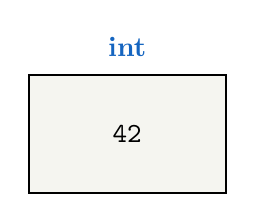
\begin{tikzpicture}
  \node[draw, thick, minimum width=2.5cm, minimum height=1.5cm, fill=codebg] (box) {};
  \node[above=0.1cm of box, font=\bfseries\color{accent}] {int};
  \node at (box.center) {\texttt{42}};
\end{tikzpicture}
\end{center}
\vspace{0.3em}
The label says what \emph{kind} of thing is inside.\\
If a function expects a box labeled \texttt{int}, don't hand it one labeled \texttt{str}.
\end{frame}

% slide 9
\begin{frame}{Static vs.\ Dynamic Typing}
Two philosophies:
\vspace{0.3em}
\begin{description}
  \item[Static typing] (Java, C, Rust): Check labels \textbf{before} running.\\
    If a label is wrong, the program won't even start.
  \item[Dynamic typing] (Python, JavaScript): Check labels \textbf{while running}.\\
    If a label is wrong, the program crashes mid-way.
\end{description}
\vspace{0.3em}
\hint{Python is dynamically typed. You only discover the mistake when the code actually runs that line.}
\end{frame}

% slide 10
\begin{frame}[fragile]{Python Type Hints}
Python lets you \emph{optionally} add labels (hints):
\begin{lstlisting}
def greet(name: str) -> str:
    return "Hello, " + name
\end{lstlisting}
\vspace{0.3em}
\begin{itemize}
  \item \texttt{name: str} — ``name should be a string''
  \item \texttt{-> str} — ``this function returns a string''
\end{itemize}
But Python \textbf{doesn't enforce} these hints at runtime.\\
Tools like \texttt{mypy} check them before you run.
\end{frame}

% slide 11
\begin{frame}[fragile]{What Types Can and Can't Tell You}
Types can tell you:
\begin{itemize}
  \item ``\texttt{x} is an \texttt{int}'' — so you can add, subtract, compare it
  \item ``\texttt{f} returns a \texttt{list}'' — so you can index into the result
\end{itemize}
\vspace{0.3em}
Types \textbf{can't} tell you:
\begin{itemize}
  \item ``\texttt{x} is a \emph{positive} integer''
  \item ``this list is \emph{sorted}''
  \item ``this string is \emph{not empty}''
  \item ``this number is \emph{not zero}''
\end{itemize}
\warn{Ordinary types say \emph{what kind}, but not \emph{which values}.}
\end{frame}

% slide 12
\begin{frame}{The Gap}
\begin{center}
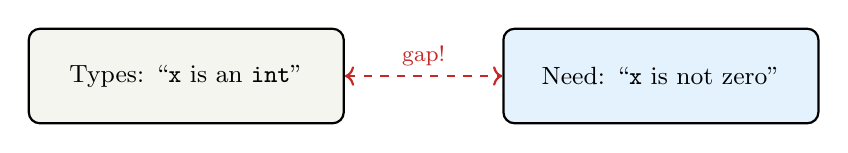
\begin{tikzpicture}[font=\small]
  \node[draw, thick, fill=codebg, rounded corners, minimum width=4cm, minimum height=1.2cm]
    (types) {Types: ``\texttt{x} is an \texttt{int}''};
  \node[draw, thick, fill=hintbg, rounded corners, minimum width=4cm, minimum height=1.2cm,
    right=2cm of types] (need) {Need: ``\texttt{x} is not zero''};
  \draw[<->, thick, danger, dashed] (types) -- node[above, font=\footnotesize\color{danger}] {gap!} (need);
\end{tikzpicture}
\end{center}
\vspace{0.5em}
Ordinary types leave a \textbf{gap} between what they guarantee\\
and what the code actually needs.
\hint{Refinement types close this gap.}
\end{frame}

% slide 13
\begin{frame}{Analogy: Airline Boarding}
\begin{itemize}
  \item \textbf{Type} = ``You have a boarding pass'' (you're a passenger)
  \item \textbf{Refinement} = ``Your boarding pass is for \emph{this flight}, \emph{this seat}''
\end{itemize}
\vspace{0.5em}
Having \emph{a} boarding pass isn't enough.\\
It has to be the \emph{right} boarding pass.
\vspace{0.5em}

Same with code: having \emph{an} int isn't enough.\\
It has to be the \emph{right kind} of int (nonzero, positive, in range, \ldots).
\end{frame}

% slide 14
\begin{frame}[fragile]{A Bug That Types Miss}
\begin{lstlisting}
def average(total: int, count: int) -> float:
    return total / count   # What if count is 0?
\end{lstlisting}
\vspace{0.3em}
\begin{itemize}
  \item \texttt{mypy} says: \textcolor{safe}{\checkmark} types are fine (\texttt{int / int} $\to$ \texttt{float})
  \item Reality: \textcolor{danger}{\texttimes} crashes when \texttt{count = 0}
\end{itemize}
\vspace{0.3em}
The type system sees ``two ints'' and says OK.\\
But the \emph{value} of \texttt{count} matters, and types don't track values.
\end{frame}

% slide 15
\begin{frame}[fragile]{Another Bug Types Miss}
\begin{lstlisting}
def first_word(text: str) -> str:
    return text.split()[0]  # What if text is ""?
\end{lstlisting}
\vspace{0.3em}
\begin{itemize}
  \item \texttt{mypy}: \textcolor{safe}{\checkmark} str in, str out
  \item Reality: \textcolor{danger}{\texttimes} \texttt{IndexError} when \texttt{text = ""}
\end{itemize}
\vspace{0.3em}
The type says ``it's a string.'' But we need ``it's a \emph{nonempty} string.''
\end{frame}

% slide 16
\begin{frame}[fragile]{Yet Another Bug Types Miss}
\begin{lstlisting}
def get_element(items: list, index: int):
    return items[index]  # What if index >= len(items)?
\end{lstlisting}
\vspace{0.3em}
\begin{itemize}
  \item Types say: list + int $\to$ OK
  \item Reality: \texttt{IndexError} if index is out of bounds
\end{itemize}
We need: ``\texttt{index} is between 0 and \texttt{len(items) - 1}.''
\end{frame}

% slide 17
\begin{frame}{The Pattern}
All three bugs have the same shape:
\vspace{0.3em}
\begin{enumerate}
  \item The \textbf{type} is correct (\texttt{int}, \texttt{str}, \texttt{list})
  \item But the code needs \textbf{more} than just the type
  \item It needs a \textbf{promise about the value}
\end{enumerate}
\vspace{0.5em}
\begin{center}
\begin{tabular}{ll}
\textbf{Bug} & \textbf{Missing promise} \\
\hline
Division by zero   & \texttt{count != 0} \\
Empty string       & \texttt{len(text) > 0} \\
Index out of bounds & \texttt{0 <= i < len(items)} \\
\end{tabular}
\end{center}
\end{frame}

% slide 18
\begin{frame}{Types Are Not Enough}
\begin{center}
\Large\bfseries
Types catch wrong \emph{kinds} of values.\\[0.5em]
But most real bugs are wrong \emph{values}\\
of the right kind.
\end{center}
\end{frame}

% slide 19
\begin{frame}{What We Need}
A way to say:
\begin{itemize}
  \item ``This is an \texttt{int} \textbf{and it's not zero}''
  \item ``This is a \texttt{str} \textbf{and it's not empty}''
  \item ``This is an \texttt{int} \textbf{and} $0 \le \texttt{i} < \texttt{len(items)}$''
  \item ``This is a \texttt{list} \textbf{and it's sorted}''
\end{itemize}
\vspace{0.5em}
In other words: \textbf{type + promise about the value}.
\hint{This is exactly what a \emph{refinement type} is.}
\end{frame}

% slide 20
\begin{frame}{Section Summary}
\begin{itemize}
  \item A \textbf{value} is a piece of data
  \item A \textbf{type} names the \emph{kind} of data (\texttt{int}, \texttt{str}, \ldots)
  \item Types catch some errors, but miss bugs about \emph{which} values
  \item We need something stronger: \textbf{type + promise}
\end{itemize}
\vspace{0.3em}
\begin{center}
\textbf{Next:} Refinement Types --- types with promises attached.
\end{center}
\end{frame}

% ═══════════════════════════════════════════════════════════
% SECTION III — REFINEMENT TYPES  (slides 21-40)
% ═══════════════════════════════════════════════════════════
\section{Refinement Types}

% slide 21
\begin{frame}{What Is a Refinement Type?}
\textbf{Refinement type} = ordinary type \textbf{+} a promise about the value.
\vspace{0.5em}
\begin{center}
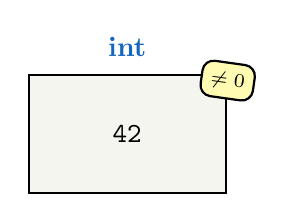
\begin{tikzpicture}
  \node[draw, thick, minimum width=2.5cm, minimum height=1.5cm, fill=codebg] (box) {};
  \node[above=0.1cm of box, font=\bfseries\color{accent}] {int};
  \node at (box.center) {\texttt{42}};
  \node[draw, thick, fill=yellow!30, rounded corners, font=\scriptsize,
    below right=-0.2cm and -0.3cm of box.north east, rotate=-8] {$\neq 0$};
\end{tikzpicture}
\end{center}
\vspace{0.3em}
The box label says ``int.'' The sticky note adds ``and it's not zero.''
\end{frame}

% slide 22
\begin{frame}{Notation (Informal)}
We'll write refinement types like this:
\vspace{0.5em}
\begin{center}
\texttt{int} where \texttt{x != 0}
\end{center}
\vspace{0.3em}
Read it as: ``an integer \texttt{x} such that \texttt{x} is not zero.''
\vspace{0.5em}

More examples:
\begin{itemize}
  \item \texttt{str} where \texttt{len(s) > 0} — a nonempty string
  \item \texttt{list} where \texttt{len(L) <= 100} — a list with at most 100 elements
  \item \texttt{float} where \texttt{0.0 <= x <= 1.0} — a probability
\end{itemize}
\end{frame}

% slide 23
\begin{frame}{Refinements Are Everywhere (You Just Don't Write Them)}
When you write:
\vspace{0.3em}
\begin{itemize}
  \item \texttt{total / count} — you're \emph{assuming} \texttt{count != 0}
  \item \texttt{items[i]} — you're \emph{assuming} \texttt{0 <= i < len(items)}
  \item \texttt{result.strip()} — you're \emph{assuming} \texttt{result is not None}
  \item \texttt{sorted\_list[0]} — you're \emph{assuming} the list isn't empty
\end{itemize}
\vspace{0.3em}
Every indexing, every division, every method call has a \textbf{hidden promise}.\\
You just never write it down.
\end{frame}

% slide 24
\begin{frame}{The Sticky-Note Analogy}
\begin{center}
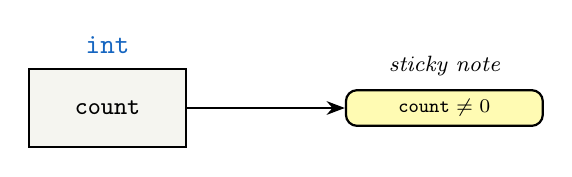
\begin{tikzpicture}[font=\small, node distance=0.5cm]
  \node[draw, thick, fill=codebg, minimum width=2cm, minimum height=1cm] (b1) {\texttt{count}};
  \node[above=0.05cm of b1, font=\bfseries\color{accent}] {\texttt{int}};

  \node[draw, thick, fill=yellow!30, rounded corners, font=\scriptsize,
    right=2cm of b1, minimum width=2.5cm] (s1) {$\texttt{count} \neq 0$};
  \node[above=0.05cm of s1, font=\footnotesize\itshape] {sticky note};

  \draw[-{Stealth}, thick] (b1) -- (s1);
\end{tikzpicture}
\end{center}
\vspace{0.5em}
\begin{itemize}
  \item The \textbf{box} = the variable and its type
  \item The \textbf{sticky note} = extra promise (refinement)
  \item Together = a refinement type
\end{itemize}
\end{frame}

% slide 25
\begin{frame}{One Value, Many Possible Refinements}
The number \texttt{42} satisfies \emph{many} refinements at once:
\vspace{0.3em}
\begin{itemize}
  \item \texttt{x != 0} \quad\textcolor{safe}{\checkmark}
  \item \texttt{x > 0} \quad\textcolor{safe}{\checkmark}
  \item \texttt{x < 100} \quad\textcolor{safe}{\checkmark}
  \item \texttt{x \% 2 == 0} \quad\textcolor{safe}{\checkmark} (it's even)
  \item \texttt{x == 42} \quad\textcolor{safe}{\checkmark} (the most precise)
\end{itemize}
\vspace{0.3em}
Refinements form a \textbf{spectrum} from vague (``it's an int'') to precise (``it's exactly 42'').
\end{frame}

% slide 26
\begin{frame}{Stronger and Weaker Promises}
Some promises \emph{imply} others:
\vspace{0.3em}
\begin{center}
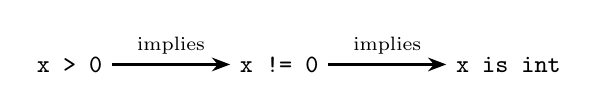
\begin{tikzpicture}[>=Stealth, font=\small, node distance=1.5cm]
  \node (a) {\texttt{x > 0}};
  \node[right=of a] (b) {\texttt{x != 0}};
  \node[right=of b] (c) {\texttt{x is int}};
  \draw[->, thick] (a) -- node[above, font=\scriptsize] {implies} (b);
  \draw[->, thick] (b) -- node[above, font=\scriptsize] {implies} (c);
\end{tikzpicture}
\end{center}
\vspace{0.3em}
If \texttt{x > 0}, then automatically \texttt{x != 0}.\\
A \textbf{stronger} promise gives you more guarantees.\\
A \textbf{weaker} promise is easier to satisfy.
\end{frame}

% slide 27
\begin{frame}[fragile]{Refinements on Different Types}
Refinements work on \emph{any} type:
\vspace{0.2em}

{\small
\begin{tabular}{@{}lll@{}}
\textbf{Type} & \textbf{Refinement} & \textbf{Meaning} \\
\hline
\texttt{int}   & \texttt{x > 0}              & positive integer \\
\texttt{str}   & \texttt{len(s) > 0}         & nonempty string \\
\texttt{list}  & \texttt{sorted(L) == L}     & sorted list \\
\texttt{dict}  & \texttt{"name" in d}        & dict with a ``name'' key \\
\texttt{float} & \texttt{not math.isnan(x)}  & not-NaN float \\
\texttt{file}  & \texttt{f.closed == False}  & open file handle \\
\end{tabular}}
\end{frame}

% slide 28
\begin{frame}{Compound Refinements}
You can combine multiple promises:
\vspace{0.5em}
\begin{center}
\texttt{int} where \texttt{x > 0} \textbf{and} \texttt{x < 100}
\end{center}
\vspace{0.3em}
``A positive integer less than 100.''
\vspace{0.5em}

\begin{center}
\texttt{list} where \texttt{len(L) > 0} \textbf{and} \texttt{sorted(L) == L}
\end{center}
\vspace{0.3em}
``A nonempty, sorted list.''
\hint{More promises = more precise = catches more bugs.}
\end{frame}

% slide 29
\begin{frame}[fragile]{Where Refinements Come From}
Refinements arise naturally from your code:
\begin{lstlisting}
if count > 0:           # after this line:
    avg = total / count # count has refinement: > 0
\end{lstlisting}
\vspace{0.3em}
\begin{lstlisting}
if result is not None:  # after this line:
    print(result.upper())  # result: not None
\end{lstlisting}
\vspace{0.3em}
Every \texttt{if}-statement \textbf{creates} a refinement inside its branch.
\end{frame}

% slide 30
\begin{frame}{Guards Create Refinements}
\begin{center}
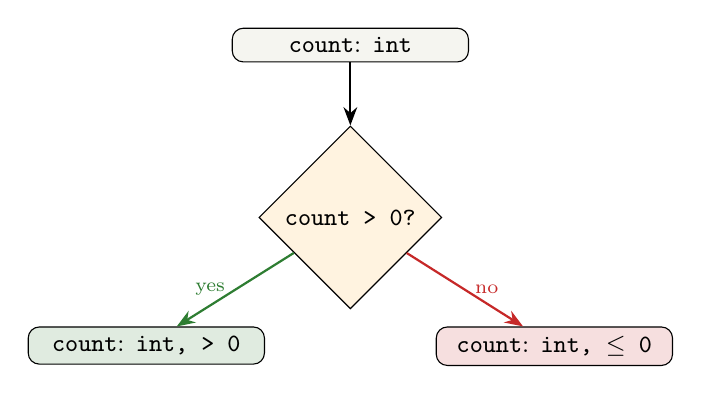
\begin{tikzpicture}[>=Stealth, font=\small]
  \node[draw, rounded corners, fill=codebg, minimum width=3cm] (before)
    {\texttt{count}: \texttt{int}};
  \node[draw, diamond, fill=warnbg, below=0.8cm of before, minimum width=2cm] (guard)
    {\texttt{count > 0?}};
  \node[draw, rounded corners, fill=safe!15, below left=0.8cm and 0.5cm of guard, minimum width=3cm] (yes)
    {\texttt{count}: \texttt{int, > 0}};
  \node[draw, rounded corners, fill=danger!15, below right=0.8cm and 0.5cm of guard, minimum width=3cm] (no)
    {\texttt{count}: \texttt{int, $\le$ 0}};
  \draw[->, thick] (before) -- (guard);
  \draw[->, thick, safe] (guard) -- node[left, font=\scriptsize] {yes} (yes);
  \draw[->, thick, danger] (guard) -- node[right, font=\scriptsize] {no} (no);
\end{tikzpicture}
\end{center}
An \texttt{if}-test \textbf{splits} a type into two refined versions.
\end{frame}

% slide 31
\begin{frame}[fragile]{Function Inputs Have Refinements}
What a function \emph{needs} from its inputs is a refinement:
\begin{lstlisting}
def binary_search(arr, target):
    # NEEDS: arr is sorted
    lo, hi = 0, len(arr) - 1
    ...
\end{lstlisting}
\vspace{0.3em}
The function works correctly \emph{only if} \texttt{arr} is sorted.\\
That's a refinement on the input: \texttt{list} where \texttt{sorted(arr) == arr}.
\end{frame}

% slide 32
\begin{frame}[fragile]{Function Outputs Have Refinements}
What a function \emph{guarantees} about its output is also a refinement:
\begin{lstlisting}
def abs_val(x):
    if x < 0:
        return -x
    return x
    # GUARANTEES: result >= 0
\end{lstlisting}
\vspace{0.3em}
The output has refinement: \texttt{int} where \texttt{result >= 0}.
\end{frame}

% slide 33
\begin{frame}{Inputs vs.\ Outputs}
\begin{center}
\begin{tabular}{@{}lll@{}}
            & \textbf{Input refinement} & \textbf{Output refinement} \\
\hline
\textbf{Who writes it?} & The caller must provide it & The function must ensure it \\
\textbf{Who benefits?}  & The function uses it & The caller uses it \\
\textbf{Analogy}        & ``Bring your passport'' & ``Here is your visa'' \\
\end{tabular}
\end{center}
\vspace{0.3em}
A function is a \textbf{contract}: I need \emph{this}, and in return I give you \emph{that}.
\end{frame}

% slide 34
\begin{frame}[fragile]{A Chain of Promises}
When functions call each other, promises chain:
\begin{lstlisting}
def get_count():    # returns: int (might be 0)
    return len(data)

def average():
    c = get_count() # c: int (might be 0)
    return total / c  # NEEDS: c != 0   <-- PROBLEM!
\end{lstlisting}
\vspace{0.3em}
\texttt{get\_count} promises ``an int.''\\
\texttt{average} needs ``an int that isn't zero.''\\
The promise isn't strong enough.
\end{frame}

% slide 35
\begin{frame}{Refinements Flow Through the Program}
\begin{center}
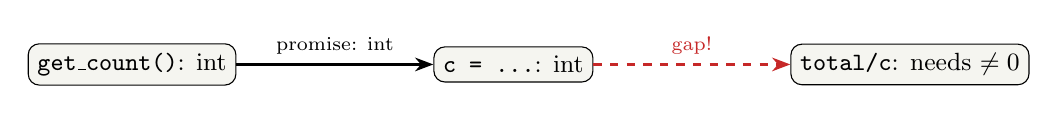
\begin{tikzpicture}[>=Stealth, font=\small, node distance=2.5cm]
  \node[draw, rounded corners, fill=codebg] (a) {\texttt{get\_count()}: int};
  \node[draw, rounded corners, fill=codebg, right=of a] (b) {\texttt{c = ...}: int};
  \node[draw, rounded corners, fill=codebg, right=of b] (c) {\texttt{total/c}: needs $\neq 0$};
  \draw[->, thick] (a) -- node[above, font=\scriptsize] {promise: int} (b);
  \draw[->, thick, danger, dashed] (b) -- node[above, font=\scriptsize\color{danger}] {gap!} (c);
\end{tikzpicture}
\end{center}
\vspace{0.3em}
Refinements \textbf{flow} from one place to the next.\\
When the flow breaks --- when what's provided doesn't meet what's needed --- that's a bug.
\end{frame}

% slide 36
\begin{frame}{Two Sides of Every Connection}
At every point where data flows from A to B:
\vspace{0.3em}
\begin{center}
\begin{tabular}{@{}ll@{}}
\textbf{Available} (what A provides) & \texttt{int} \\
\textbf{Required} (what B needs)     & \texttt{int} where \texttt{x != 0} \\
\end{tabular}
\end{center}
\vspace{0.3em}
\textbf{Bug} $=$ Required is \emph{stronger} than Available.\\
\textbf{Safe} $=$ Available is \emph{at least as strong as} Required.
\end{frame}

% slide 37
\begin{frame}[fragile]{Making It Safe with a Guard}
\begin{lstlisting}
def average():
    c = get_count()   # c: int (might be 0)
    if c == 0:
        return 0.0    # early exit: safe
    return total / c  # NOW c: int, != 0  -- safe!
\end{lstlisting}
\vspace{0.3em}
The \texttt{if} guard \textbf{creates} the missing refinement.\\
After the guard, we \emph{know} \texttt{c != 0}, so division is safe.
\end{frame}

% slide 38
\begin{frame}{Why Not Just Use Tests?}
Tests check \emph{specific} inputs:
\begin{itemize}
  \item \texttt{test\_average(10, 2)} $\to$ 5.0 \textcolor{safe}{\checkmark}
  \item \texttt{test\_average(0, 0)} $\to$ crash \textcolor{danger}{\texttimes}
\end{itemize}
\vspace{0.3em}
But you have to \emph{think of} the bad input.\\
If you forgot to test \texttt{count = 0}, the test suite passes and the bug hides.
\vspace{0.3em}

Refinement types check \emph{all possible} inputs by reasoning about promises, not examples.
\warn{Tests: ``these 5 inputs work.'' Refinements: ``\emph{every} input works (or here's one that doesn't).''}
\end{frame}

% slide 39
\begin{frame}{Refinement Types: The Key Idea}
\begin{center}
\Large
\textbf{Type} = what kind of box\\[0.4em]
\textbf{Refinement} = a sticky note on the box\\[0.4em]
\textbf{Bug} = a sticky note that's missing\\
where the next function needs one
\end{center}
\end{frame}

% slide 40
\begin{frame}{Section Summary}
\begin{itemize}
  \item A \textbf{refinement type} = type + promise about the value
  \item Refinements arise from \texttt{if}-guards, function contracts, computations
  \item They flow through the program along data paths
  \item A bug = a place where the \textbf{available} refinement is weaker than the \textbf{required} one
  \item Tests check examples; refinements check \emph{all} values
\end{itemize}
\vspace{0.3em}
\begin{center}
\textbf{Next:} What happens when promises break?
\end{center}
\end{frame}

% ═══════════════════════════════════════════════════════════
% SECTION IV — THE PROBLEM: PROMISES BREAK  (slides 41-60)
% ═══════════════════════════════════════════════════════════
\section{The Problem: Promises Break}

% slide 41
\begin{frame}{Programs Have Many Parts}
A real program isn't one function --- it's \textbf{hundreds} of functions calling each other.
\vspace{0.3em}
\begin{center}
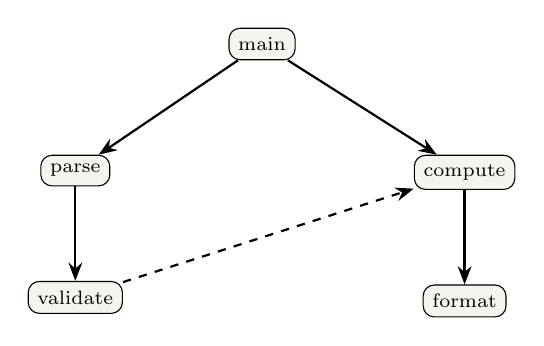
\begin{tikzpicture}[>=Stealth, font=\scriptsize, node distance=1.2cm and 1.5cm]
  \node[draw, rounded corners, fill=codebg] (a) {main};
  \node[draw, rounded corners, fill=codebg, below left=of a] (b) {parse};
  \node[draw, rounded corners, fill=codebg, below right=of a] (c) {compute};
  \node[draw, rounded corners, fill=codebg, below=of b] (d) {validate};
  \node[draw, rounded corners, fill=codebg, below=of c] (e) {format};
  \draw[->, thick] (a) -- (b); \draw[->, thick] (a) -- (c);
  \draw[->, thick] (b) -- (d); \draw[->, thick] (c) -- (e);
  \draw[->, thick, dashed] (d) -- (c);
\end{tikzpicture}
\end{center}
Each arrow is a place where data flows --- and promises must match.
\end{frame}

% slide 42
\begin{frame}{Each Part Makes Its Own Promises}
\begin{center}
\begin{tabular}{@{}lll@{}}
\textbf{Function} & \textbf{Promises about input} & \textbf{Promises about output} \\
\hline
\texttt{parse}    & takes a string & returns a dict \\
\texttt{validate} & takes a dict   & returns a dict with ``name'' key \\
\texttt{compute}  & takes a dict with ``name'' & returns an int $> 0$ \\
\texttt{format}   & takes an int $> 0$ & returns a string \\
\end{tabular}
\end{center}
\vspace{0.3em}
Each function has its own input and output promises (refinements).
\end{frame}

% slide 43
\begin{frame}{The Handoff Problem}
When function A calls function B:
\vspace{0.5em}
\begin{center}
A's \textbf{output promise} must be $\ge$ B's \textbf{input requirement}
\end{center}
\vspace{0.5em}
If A promises ``an int'' but B needs ``an int $> 0$'':
\begin{itemize}
  \item A might hand over \texttt{0} or \texttt{-5}
  \item B will crash or produce wrong results
  \item The \textbf{handoff} is the problem
\end{itemize}
\end{frame}

% slide 44
\begin{frame}{Visualizing a Promise Mismatch}
\begin{center}
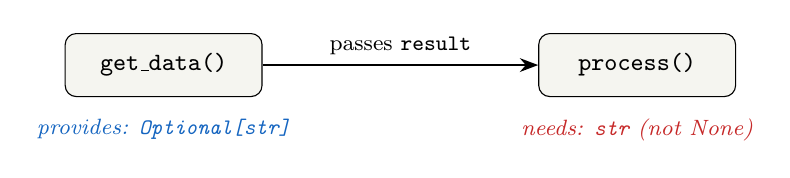
\begin{tikzpicture}[>=Stealth, font=\small, node distance=3.5cm]
  \node[draw, rounded corners, fill=codebg, minimum width=2.5cm, minimum height=0.8cm]
    (A) {\texttt{get\_data()}};
  \node[draw, rounded corners, fill=codebg, minimum width=2.5cm, minimum height=0.8cm, right=of A]
    (B) {\texttt{process()}};
  \draw[->, thick] (A) -- node[above]{\footnotesize passes \texttt{result}} (B);
  \node[below=0.15cm of A, text=accent, font=\footnotesize\itshape] {provides: \texttt{Optional[str]}};
  \node[below=0.15cm of B, text=danger, font=\footnotesize\itshape] {needs: \texttt{str} (not None)};
\end{tikzpicture}
\end{center}
\vspace{0.3em}
\texttt{get\_data()} might return \texttt{None}.\\
\texttt{process()} calls \texttt{.strip()} on it --- crash!
\warn{The arrow between the two functions is where the bug lives.}
\end{frame}

% slide 45
\begin{frame}[fragile]{Example 1: Division by Zero}
\begin{lstlisting}
def get_count(data):
    return len(data)    # might be 0

def average(data, total):
    count = get_count(data)
    return total / count  # BOOM if count == 0
\end{lstlisting}
\vspace{0.3em}
\begin{tabular}{@{}ll@{}}
Available: & \texttt{int} (could be anything) \\
Required:  & \texttt{int} where \texttt{x != 0} \\
Verdict:   & \textcolor{danger}{Promise too weak} \\
\end{tabular}
\end{frame}

% slide 46
\begin{frame}[fragile]{Example 2: None Dereference}
\begin{lstlisting}
def find_user(db, name):
    return db.get(name)  # might be None

def greet(db, name):
    user = find_user(db, name)
    print("Hi " + user.display_name)  # BOOM if None
\end{lstlisting}
\vspace{0.3em}
\begin{tabular}{@{}ll@{}}
Available: & \texttt{Optional[User]} (might be None) \\
Required:  & \texttt{User} (not None) \\
Verdict:   & \textcolor{danger}{Promise too weak} \\
\end{tabular}
\end{frame}

% slide 47
\begin{frame}[fragile]{Example 3: Index Out of Bounds}
\begin{lstlisting}
def get_first(items):
    return items[0]     # BOOM if items is empty

def process(data):
    if data:
        items = parse(data)
    else:
        items = []
    return get_first(items)  # items might be []
\end{lstlisting}
\vspace{0.3em}
\begin{tabular}{@{}ll@{}}
Available: & \texttt{list} (might be empty) \\
Required:  & \texttt{list} where \texttt{len(L) > 0} \\
\end{tabular}
\end{frame}

% slide 48
\begin{frame}[fragile]{Example 4: Key Error}
\begin{lstlisting}
def get_setting(config, key):
    return config[key]  # BOOM if key not in config

settings = {"host": "localhost"}
port = get_setting(settings, "port")  # KeyError!
\end{lstlisting}
\vspace{0.3em}
\begin{tabular}{@{}ll@{}}
Available: & \texttt{dict} (might not have that key) \\
Required:  & \texttt{dict} where \texttt{key in d} \\
\end{tabular}
\end{frame}

% slide 49
\begin{frame}[fragile]{Example 5: Type Mismatch}
\begin{lstlisting}
def build_message(name, age):
    return "Hello " + name + " age " + age
    # BOOM if age is int, not str
\end{lstlisting}
\vspace{0.3em}
\begin{tabular}{@{}ll@{}}
Available: & \texttt{int} (from caller) \\
Required:  & \texttt{str} (for concatenation) \\
Verdict:   & \textcolor{danger}{Carrier mismatch --- entirely wrong type} \\
\end{tabular}
\end{frame}

% slide 50
\begin{frame}{The Common Shape}
Every example has the same shape:
\vspace{0.5em}
\begin{enumerate}
  \item Function A produces a value with promise $P$
  \item Function B needs a value with promise $Q$
  \item $P$ does not imply $Q$
  \item \textbf{Bug.}
\end{enumerate}
\vspace{0.5em}
\hint{$P \not\Rightarrow Q$ at a connection = a bug.\\
$P \Rightarrow Q$ at every connection = no bugs.}
\end{frame}

% slide 51
\begin{frame}{Beyond Simple Functions}
Promise mismatches happen not just between functions, but:
\vspace{0.3em}
\begin{itemize}
  \item Between \textbf{branches}: the \texttt{if}-branch sets a variable, the \texttt{else}-branch doesn't
  \item Between \textbf{loop iterations}: a value changes inside the loop
  \item Between \textbf{modules}: one file exports a value, another imports it
  \item Between \textbf{threads}: two threads access the same data
\end{itemize}
\vspace{0.3em}
Anywhere data flows from one place to another, promises must match.
\end{frame}

% slide 52
\begin{frame}[fragile]{Branch Mismatch}
\begin{lstlisting}
def process(flag):
    if flag:
        x = 42
    # else: x is never assigned!
    return x   # BOOM if flag is False
\end{lstlisting}
\vspace{0.3em}
One branch promises ``x exists.'' The other branch makes no such promise.\\
After the \texttt{if}, we can't be sure \texttt{x} is defined.
\end{frame}

% slide 53
\begin{frame}[fragile]{Loop Mismatch}
\begin{lstlisting}
def countdown(n):
    while n > 0:
        pass  # oops, n never changes!
    return n
\end{lstlisting}
\vspace{0.3em}
Before the loop: \texttt{n > 0}.\\
The loop body should make progress toward \texttt{n <= 0}.\\
But it doesn't --- so the loop never ends.
\warn{Non-termination = a promise about ``eventually finishing'' that's broken.}
\end{frame}

% slide 54
\begin{frame}[fragile]{Resource Mismatch}
\begin{lstlisting}
f = open("data.txt", "r")
data = f.read()
f.close()
print(f.read())  # BOOM: file is already closed!
\end{lstlisting}
\vspace{0.3em}
After \texttt{f.close()}: the promise ``f is open'' becomes ``f is closed.''\\
\texttt{f.read()} needs ``f is open'' --- mismatch!
\end{frame}

% slide 55
\begin{frame}[fragile]{Thread Mismatch}
\begin{lstlisting}
shared = []
def worker1():
    shared.append(1)  # no lock!
def worker2():
    shared.append(2)  # no lock!
\end{lstlisting}
\vspace{0.3em}
Both threads promise ``I can modify \texttt{shared}.''\\
But neither promises ``I have exclusive access.''\\
Result: data race.
\end{frame}

% slide 56
\begin{frame}{How Many Connections Does a Program Have?}
\begin{center}
\begin{tabular}{@{}lr@{}}
\textbf{Program size} & \textbf{Approximate connections} \\
\hline
10-line script     & $\sim$5 \\
100-line module    & $\sim$50 \\
1,000-line package & $\sim$500 \\
10,000-line app    & $\sim$5,000 \\
\end{tabular}
\end{center}
\vspace{0.3em}
Every connection is a place where promises must match.\\
Checking them all by hand is impossible.\\
We need \textbf{automation}.
\end{frame}

% slide 57
\begin{frame}{Why Is This Hard?}
\begin{itemize}
  \item Promises are \textbf{implicit} --- programmers rarely write them down
  \item They \textbf{flow} through many layers of function calls
  \item They \textbf{change} at every \texttt{if}-branch, loop iteration, and exception handler
  \item A bug might involve a chain of 5+ functions
\end{itemize}
\vspace{0.3em}
We need a \textbf{systematic framework} for:
\begin{enumerate}
  \item Discovering what each part promises
  \item Checking that adjacent promises agree
  \item Reporting exactly where they don't
\end{enumerate}
\end{frame}

% slide 58
\begin{frame}{What Would a Solution Look Like?}
Imagine a tool that could:
\vspace{0.3em}
\begin{enumerate}
  \item Scan your code automatically
  \item Find every ``observation point'' (variable, function input, branch, \ldots)
  \item Record the promise at each point
  \item Check every connection: does promise A imply promise B?
  \item Report mismatches as bugs, with exact locations
\end{enumerate}
\vspace{0.5em}
\hint{This is exactly what DepPy does. And the theory behind it is the ``sheaf'' idea.}
\end{frame}

% slide 59
\begin{frame}{Preview: The Sheaf Idea in One Sentence}
\begin{center}
\Large\bfseries
Local promises that fit together consistently\\
form a global guarantee.\\[0.5em]
\normalsize
Local promises that \emph{don't} fit together\\
reveal exactly where the bugs are.
\end{center}
\end{frame}

% slide 60
\begin{frame}{Section Summary}
\begin{itemize}
  \item Programs have many parts, each with its own promises
  \item Where parts connect, promises must \textbf{agree}
  \item Mismatches = bugs (div-by-zero, null deref, OOB, \ldots)
  \item Mismatches happen between functions, branches, loops, threads
  \item Checking by hand doesn't scale --- we need a framework
\end{itemize}
\vspace{0.3em}
\begin{center}
\textbf{Next:} The Jigsaw Puzzle --- a visual way to think about this.
\end{center}
\end{frame}

% ═══════════════════════════════════════════════════════════
% SECTION V — THE JIGSAW PUZZLE (SHEAF IDEA)  (slides 61-85)
% ═══════════════════════════════════════════════════════════
\section{The Jigsaw Puzzle}

% slide 61
\begin{frame}{The Central Analogy}
\begin{center}
\Large
Your program is a \textbf{jigsaw puzzle}.\\[0.5em]
\normalsize
Each piece = one part of your code.\\
Each edge = a connection between parts.\\
The picture on each piece = the promise it makes.
\end{center}
\end{frame}

% slide 62
\begin{frame}{Pieces}
A \textbf{piece} is any chunk of code that has its own promise:
\vspace{0.3em}
\begin{itemize}
  \item A function
  \item One branch of an \texttt{if}/\texttt{else}
  \item A single variable at a particular point
  \item A loop body
  \item A return statement
\end{itemize}
\vspace{0.3em}
Each piece ``knows'' something about the values passing through it.
\end{frame}

% slide 63
\begin{frame}{Edges}
An \textbf{edge} is where two pieces touch --- where data flows from one to another:
\vspace{0.3em}
\begin{itemize}
  \item Function A calls Function B $\to$ edge at the call site
  \item \texttt{if}-branch flows into code after the \texttt{if} $\to$ edge at the join
  \item Loop iteration $n$ flows into iteration $n+1$ $\to$ edge at the loop header
  \item Module A imports from Module B $\to$ edge at the import
\end{itemize}
\end{frame}

% slide 64
\begin{frame}{Pictures on Pieces}
The ``picture'' on a piece is its \textbf{local promise} (refinement):
\vspace{0.5em}
\begin{center}
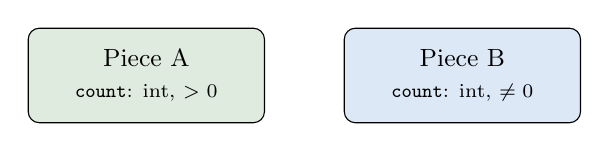
\begin{tikzpicture}[font=\small]
  \node[draw, fill=safe!15, rounded corners, minimum width=3cm, minimum height=1.2cm,
    align=center] (P1) {Piece A\\{\scriptsize\texttt{count}: int, $> 0$}};
  \node[draw, fill=accent!15, rounded corners, minimum width=3cm, minimum height=1.2cm,
    align=center, right=1cm of P1] (P2) {Piece B\\{\scriptsize\texttt{count}: int, $\neq 0$}};
\end{tikzpicture}
\end{center}
\vspace{0.3em}
Piece A says: ``count is a positive integer.''\\
Piece B says: ``count is a nonzero integer.''
\end{frame}

% slide 65
\begin{frame}{Matching Edges}
Two pieces \textbf{match} at their shared edge if:
\vspace{0.3em}
\begin{center}
Piece A's promise \textbf{implies} Piece B's requirement
\end{center}
\vspace{0.5em}
\begin{center}
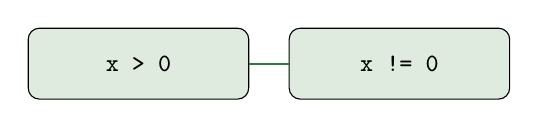
\begin{tikzpicture}[font=\small]
  \node[draw, fill=safe!15, rounded corners, minimum width=2.8cm, minimum height=0.9cm]
    (P1) {\texttt{x > 0}};
  \node[draw, fill=safe!15, rounded corners, minimum width=2.8cm, minimum height=0.9cm,
    right=0.5cm of P1] (P2) {\texttt{x != 0}};
  \draw[thick, safe] (P1) -- node[above, font=\scriptsize\bfseries\color{safe}] {\checkmark} (P2);
\end{tikzpicture}
\end{center}
\vspace{0.3em}
\texttt{x > 0} implies \texttt{x != 0} $\to$ edge matches $\to$ \textcolor{safe}{safe}.
\end{frame}

% slide 66
\begin{frame}{Mismatching Edges}
Two pieces \textbf{don't match} when the promise is too weak:
\vspace{0.5em}
\begin{center}
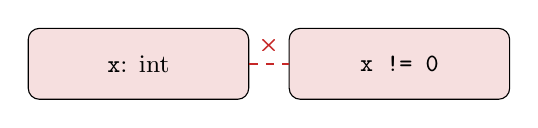
\begin{tikzpicture}[font=\small]
  \node[draw, fill=danger!15, rounded corners, minimum width=2.8cm, minimum height=0.9cm]
    (P1) {\texttt{x}: int};
  \node[draw, fill=danger!15, rounded corners, minimum width=2.8cm, minimum height=0.9cm,
    right=0.5cm of P1] (P2) {\texttt{x != 0}};
  \draw[thick, danger, dashed] (P1) -- node[above, font=\scriptsize\bfseries\color{danger}] {\texttimes} (P2);
\end{tikzpicture}
\end{center}
\vspace{0.3em}
``int'' does NOT imply ``int, not zero'' $\to$ edge mismatches $\to$ \textcolor{danger}{bug}.
\end{frame}

% slide 67
\begin{frame}{The Puzzle Is Complete When\ldots}
\begin{center}
\Large\bfseries
Every edge matches.
\end{center}
\vspace{0.5em}
\normalsize
If all neighboring pieces agree at every shared edge, the puzzle fits together perfectly.\\[0.3em]
This means: \textbf{no bugs} (of the kinds we're checking).
\hint{All edges match $\Rightarrow$ all local promises are globally consistent $\Rightarrow$ safe program.}
\end{frame}

% slide 68
\begin{frame}{The Puzzle Has a Hole When\ldots}
\begin{center}
\Large\bfseries
Some edge doesn't match.
\end{center}
\vspace{0.5em}
\normalsize
If even one pair of neighboring pieces disagree, the puzzle has a gap.\\[0.3em]
That gap \textbf{is} the bug, and we know \textbf{exactly which edge} it is.
\end{frame}

% slide 69
\begin{frame}{A Three-Piece Example}
\begin{center}
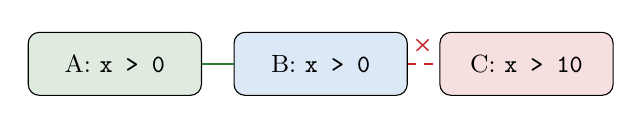
\begin{tikzpicture}[font=\small]
  \node[draw, fill=safe!15, rounded corners, minimum width=2.2cm, minimum height=0.8cm]
    (P1) {A: \texttt{x > 0}};
  \node[draw, fill=accent!15, rounded corners, minimum width=2.2cm, minimum height=0.8cm,
    right=0.4cm of P1] (P2) {B: \texttt{x > 0}};
  \node[draw, fill=danger!15, rounded corners, minimum width=2.2cm, minimum height=0.8cm,
    right=0.4cm of P2] (P3) {C: \texttt{x > 10}};
  \draw[thick, safe] (P1) -- node[above, font=\scriptsize\bfseries, text=safe] {\checkmark} (P2);
  \draw[thick, danger, dashed] (P2) -- node[above, font=\scriptsize\bfseries, text=danger] {\texttimes} (P3);
\end{tikzpicture}
\end{center}
\vspace{0.3em}
\begin{itemize}
  \item A$\to$B: \texttt{x > 0} implies \texttt{x > 0} \textcolor{safe}{\checkmark}
  \item B$\to$C: \texttt{x > 0} does NOT imply \texttt{x > 10} \textcolor{danger}{\texttimes}
\end{itemize}
The bug is at the B$\to$C edge. Not at A, not at B alone, not at C alone.
\end{frame}

% slide 70
\begin{frame}{Local vs.\ Global}
\begin{description}
  \item[Local] = what one piece promises \emph{by itself}
  \item[Global] = what the whole puzzle promises \emph{put together}
\end{description}
\vspace{0.5em}
The key insight:
\begin{center}
\textbf{You can build a global guarantee from local promises\\
if and only if all local promises agree at their edges.}
\end{center}
\end{frame}

% slide 71
\begin{frame}{This Is the Sheaf Idea}
In mathematics, this principle has a name: the \textbf{sheaf condition}.
\vspace{0.5em}
\begin{quote}
A collection of local data can be ``glued'' into one consistent global piece of data
if and only if the local pieces \textbf{agree on overlaps}.
\end{quote}
\vspace{0.5em}
We won't use the math. We'll use the jigsaw puzzle version.\\
But if you ever hear ``sheaf,'' think: \textbf{jigsaw puzzle}.
\end{frame}

% slide 72
\begin{frame}{The Word ``Sheaf''}
The word ``sheaf'' comes from agriculture: a bundle of wheat stalks tied together.
\vspace{0.5em}
\begin{center}
Individual stalks (local pieces) $\xrightarrow{\text{tied together}}$ one sheaf (global whole)
\end{center}
\vspace{0.5em}
In our analogy:\\
Individual promises (local) $\xrightarrow{\text{edges match}}$ one guarantee (global)
\end{frame}

% slide 73
\begin{frame}{Gluing}
When all edges match, we can \textbf{glue} the local promises into one big global promise.
\vspace{0.5em}
\begin{center}
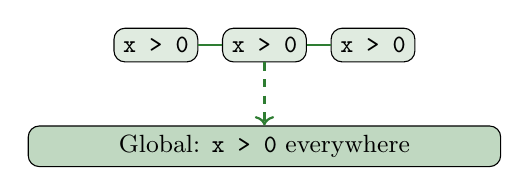
\begin{tikzpicture}[font=\small]
  \node[draw, fill=safe!15, rounded corners] (P1) {\texttt{x > 0}};
  \node[draw, fill=safe!15, rounded corners, right=0.3cm of P1] (P2) {\texttt{x > 0}};
  \node[draw, fill=safe!15, rounded corners, right=0.3cm of P2] (P3) {\texttt{x > 0}};
  \draw[thick, safe] (P1) -- (P2); \draw[thick, safe] (P2) -- (P3);

  \node[draw, fill=safe!30, rounded corners, minimum width=6cm, below=0.8cm of P2]
    (G) {Global: \texttt{x > 0} everywhere};
  \draw[->, thick, safe, dashed] (P2) -- (G);
\end{tikzpicture}
\end{center}
\hint{Gluing = combining compatible local promises into a global fact.}
\end{frame}

% slide 74
\begin{frame}{Obstruction}
When an edge \textbf{doesn't} match, we can't glue. The mismatch is called an \textbf{obstruction}.
\vspace{0.5em}
\begin{center}
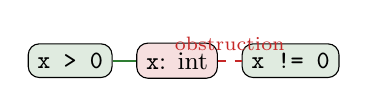
\begin{tikzpicture}[font=\small]
  \node[draw, fill=safe!15, rounded corners] (P1) {\texttt{x > 0}};
  \node[draw, fill=danger!15, rounded corners, right=0.3cm of P1] (P2) {\texttt{x}: int};
  \node[draw, fill=safe!15, rounded corners, right=0.3cm of P2] (P3) {\texttt{x != 0}};
  \draw[thick, safe] (P1) -- (P2);
  \draw[thick, danger, dashed] (P2) -- node[above, font=\scriptsize\color{danger}] {obstruction} (P3);
\end{tikzpicture}
\end{center}
\vspace{0.3em}
An obstruction = a bug, located at a specific edge.
\end{frame}

% slide 75
\begin{frame}{Why ``Obstruction'' and Not Just ``Bug''?}
Because it tells you \textbf{more} than ``there's a bug'':
\vspace{0.3em}
\begin{itemize}
  \item \textbf{Which edge} --- exactly which two pieces disagree
  \item \textbf{What's available} --- what the left piece promises
  \item \textbf{What's required} --- what the right piece needs
  \item \textbf{The gap} --- what's missing (the obstruction itself)
\end{itemize}
\vspace{0.3em}
An obstruction is a bug with a \textbf{diagnosis built in}.
\end{frame}

% slide 76
\begin{frame}{Many Puzzles, One Idea}
Different kinds of promises give different kinds of puzzles:
\vspace{0.3em}
{\small
\begin{tabular}{@{}lll@{}}
\textbf{Promise type}  & \textbf{Piece talks about} & \textbf{Mismatch =} \\
\hline
Value range       & ``x $\neq$ 0''             & division by zero \\
Nullability       & ``x is not None''          & null dereference \\
Resource state    & ``file is open''           & use after close \\
Bounds            & ``0 $\le$ i $<$ len''      & index out of bounds \\
Taint status      & ``input is sanitized''     & injection attack \\
Lock state        & ``lock is held''           & data race \\
Termination       & ``loop decreases''         & infinite loop \\
\end{tabular}}
\end{frame}

% slide 77
\begin{frame}{Analogy: City Maps}
Imagine you have \textbf{local maps} of different neighborhoods:
\vspace{0.3em}
\begin{itemize}
  \item Map A covers downtown
  \item Map B covers the waterfront
  \item Map C covers the university
\end{itemize}
\vspace{0.3em}
Where maps \textbf{overlap} (e.g., downtown meets waterfront), the streets must match.\\[0.3em]
If they do, you can glue the maps into one big city map.\\
If a street appears on one map but not the other, something's wrong.
\hint{Local maps = local promises. Overlap = shared edge. City map = global guarantee.}
\end{frame}

% slide 78
\begin{frame}{Analogy: Witness Statements}
Five witnesses describe a car accident:
\vspace{0.3em}
\begin{itemize}
  \item Each witness saw \textbf{part} of the event (local view)
  \item Where two witnesses overlap, their stories should agree
  \item If all overlaps agree, we can reconstruct what happened (global view)
  \item If two witnesses contradict, we know \textbf{exactly where} the discrepancy is
\end{itemize}
\vspace{0.3em}
Same idea, different domain. The ``sheaf condition'' appears everywhere.
\end{frame}

% slide 79
\begin{frame}{Three Steps of the Sheaf Approach}
\begin{enumerate}
  \item \textbf{Decompose}: break the program into pieces (observation points)
  \item \textbf{Record}: write down the local promise at each piece
  \item \textbf{Check edges}: for every pair of touching pieces, does promise A imply promise B?
\end{enumerate}
\vspace{0.5em}
All edges match $\Rightarrow$ glue into global guarantee $\Rightarrow$ \textcolor{safe}{safe}.\\
Some edge fails $\Rightarrow$ report obstruction $\Rightarrow$ \textcolor{danger}{bug found}.
\end{frame}

% slide 80
\begin{frame}{What ``Checking Edges'' Really Means}
For each connection from site $u$ to site $v$:
\vspace{0.3em}
\begin{enumerate}
  \item Look up the promise at $u$ (what's available)
  \item Look up the promise at $v$ (what's required)
  \item Ask: does Available $\Rightarrow$ Required?
\end{enumerate}
\vspace{0.3em}
If yes: that edge is \textcolor{safe}{safe}.\\
If no: that edge is a \textcolor{danger}{bug} --- and we report it with both promises, so the developer knows exactly what's wrong.
\end{frame}

% slide 81
\begin{frame}{Uniqueness}
The sheaf idea guarantees one more thing: if a global guarantee exists, it's \textbf{unique}.
\vspace{0.5em}
There's only \emph{one} way to glue the local promises into a global fact.\\
You can't accidentally produce two different ``global truths'' from the same local data.
\vspace{0.5em}
\hint{Uniqueness = no ambiguity. The analysis gives one definite answer.}
\end{frame}

% slide 82
\begin{frame}{The Sheaf Idea Summarized}
\begin{center}
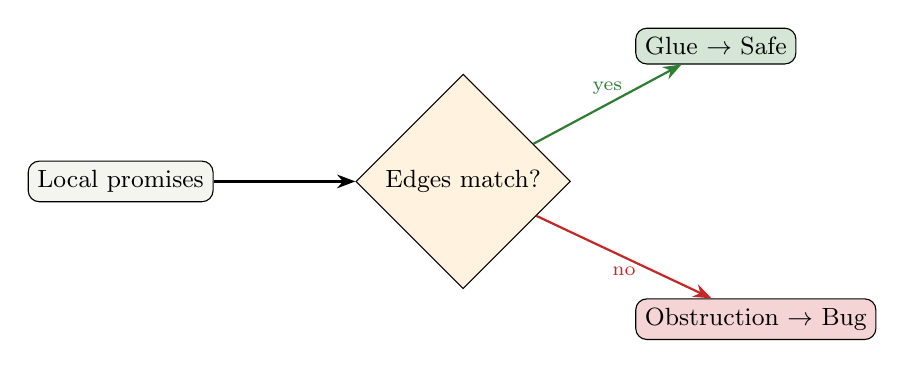
\begin{tikzpicture}[font=\small, >=Stealth, node distance=1.8cm]
  \node[draw, rounded corners, fill=codebg] (pieces) {Local promises};
  \node[draw, diamond, fill=warnbg, right=of pieces] (check) {Edges match?};
  \node[draw, rounded corners, fill=safe!20, above right=0.8cm and 1.5cm of check] (safe) {Glue $\to$ Safe};
  \node[draw, rounded corners, fill=danger!20, below right=0.8cm and 1.5cm of check] (bug) {Obstruction $\to$ Bug};
  \draw[->, thick] (pieces) -- (check);
  \draw[->, thick, safe] (check) -- node[above, font=\scriptsize] {yes} (safe);
  \draw[->, thick, danger] (check) -- node[below, font=\scriptsize] {no} (bug);
\end{tikzpicture}
\end{center}
\end{frame}

% slide 83
\begin{frame}{Why Not Just Check Everything Globally?}
Why break it into pieces? Why not analyze the whole program at once?
\vspace{0.3em}
\begin{itemize}
  \item Programs are \textbf{too big} to analyze as one unit
  \item Local analysis is \textbf{fast} (each piece is small)
  \item Edge checking is \textbf{simple} (compare two promises)
  \item You get \textbf{precise locations} for bugs (not ``somewhere in your 10,000 lines'')
\end{itemize}
\hint{``Think locally, conclude globally'' --- that's the sheaf motto.}
\end{frame}

% slide 84
\begin{frame}{Comparison with Other Approaches}
\begin{center}
{\small
\begin{tabular}{@{}lcccc@{}}
 & \textbf{Types} & \textbf{Tests} & \textbf{Linters} & \textbf{Sheaf} \\
\hline
Finds type errors     & \textcolor{safe}{\checkmark} & sometimes & \textcolor{safe}{\checkmark} & \textcolor{safe}{\checkmark} \\
Finds value errors    & \textcolor{danger}{\texttimes} & sometimes & sometimes & \textcolor{safe}{\checkmark} \\
All inputs            & \textcolor{safe}{\checkmark} & \textcolor{danger}{\texttimes} & partial & \textcolor{safe}{\checkmark} \\
Pinpoints location    & partial & \textcolor{danger}{\texttimes} & \textcolor{safe}{\checkmark} & \textcolor{safe}{\checkmark} \\
Explains \emph{why}   & \textcolor{danger}{\texttimes} & \textcolor{danger}{\texttimes} & \textcolor{danger}{\texttimes} & \textcolor{safe}{\checkmark} \\
\end{tabular}}
\end{center}
\end{frame}

% slide 85
\begin{frame}{Section Summary}
\begin{itemize}
  \item Program = jigsaw puzzle; pieces = code parts; edges = data flow
  \item Each piece has a \textbf{local promise} (refinement)
  \item Edges match $\Rightarrow$ \textbf{glue} into global guarantee $\Rightarrow$ safe
  \item Edge mismatch $\Rightarrow$ \textbf{obstruction} $\Rightarrow$ bug with exact location
  \item This is the ``sheaf condition'' --- no math needed, just the jigsaw analogy
\end{itemize}
\vspace{0.3em}
\begin{center}
\textbf{Next:} How DepPy turns this idea into a real tool.
\end{center}
\end{frame}

% ═══════════════════════════════════════════════════════════
% SECTION VI — HOW DEPPY SEES CODE (SITES)  (slides 86-110)
% ═══════════════════════════════════════════════════════════
\section{How DepPy Sees Code}

% slide 86
\begin{frame}{From Jigsaw to Real Code}
We said: ``pieces = code parts, edges = data flow.''\\[0.3em]
Now let's make that \textbf{precise}. How does DepPy actually carve up a program?
\vspace{0.5em}
\begin{center}
DepPy picks specific \textbf{observation points} in your code.\\
Each observation point is called a \textbf{site}.
\end{center}
\end{frame}

% slide 87
\begin{frame}{What Is a Site?}
A \textbf{site} is a place in your code where DepPy stops and asks:
\begin{center}
``What do I know about the data here, right now?''
\end{center}
\vspace{0.5em}
Examples of sites:
\begin{itemize}
  \item The argument \texttt{n} at the start of \texttt{def factorial(n)}
  \item The return value of a function
  \item The value of \texttt{x} right after \texttt{x = len(items)}
  \item The condition in \texttt{if x > 0}
\end{itemize}
\end{frame}

% slide 88
\begin{frame}{DepPy Has 14 Kinds of Sites}
DepPy looks at \textbf{14 different kinds} of observation points:
\vspace{0.3em}
{\small
\begin{columns}[T]
\begin{column}{0.48\textwidth}
\begin{enumerate}
  \item Argument boundary
  \item Return boundary
  \item SSA value
  \item Branch guard
  \item Call result
  \item Tensor shape
  \item Tensor order
\end{enumerate}
\end{column}
\begin{column}{0.48\textwidth}
\begin{enumerate}\setcounter{enumi}{7}
  \item Tensor indexing
  \item Heap protocol
  \item Proof
  \item Trace
  \item Error
  \item Loop header invariant
  \item Module summary
\end{enumerate}
\end{column}
\end{columns}}
\vspace{0.3em}
Don't worry --- we'll explain the important ones step by step.
\end{frame}

% slide 89
\begin{frame}[fragile]{Site 1: Argument Boundary}
Where a function \textbf{receives} its inputs.
\vspace{0.3em}
\begin{lstlisting}[language=Python]
def divide(a: int, b: int) -> float:
    # SITE: b at argument boundary
    # DepPy asks: "What do I know about b?"
    return a / b
\end{lstlisting}
\vspace{0.3em}
DepPy records: \texttt{b} has type \texttt{int}, but \textbf{no} promise that \texttt{b $\neq$ 0}.
\end{frame}

% slide 90
\begin{frame}[fragile]{Site 2: Return Boundary}
Where a function \textbf{sends back} its result.
\vspace{0.3em}
\begin{lstlisting}[language=Python]
def safe_divide(a, b):
    if b == 0:
        return 0.0   # SITE: return boundary
    return a / b      # SITE: return boundary
\end{lstlisting}
\vspace{0.3em}
DepPy records: first return always gives \texttt{0.0}.\\
Second return: \texttt{b $\neq$ 0} on this path, so division is safe.
\end{frame}

% slide 91
\begin{frame}[fragile]{Site 3: SSA Value}
A variable at a \textbf{specific point} in the code (``single static assignment'').
\vspace{0.3em}
\begin{lstlisting}[language=Python]
x = get_input()    # SITE: x = ??? (unknown)
x = abs(x)         # SITE: x >= 0  (known!)
x = x + 1          # SITE: x >= 1  (even better)
\end{lstlisting}
\vspace{0.3em}
The \emph{same variable} has \emph{different promises} at different lines.\\
DepPy tracks each one as a separate site.
\end{frame}

% slide 92
\begin{frame}[fragile]{Site 4: Branch Guard}
The \textbf{condition} in an \texttt{if} or \texttt{while} statement.
\vspace{0.3em}
\begin{lstlisting}[language=Python]
if x > 0:          # SITE: branch guard
    print(1 / x)   # safe! guard guarantees x > 0
\end{lstlisting}
\vspace{0.3em}
The branch guard creates a \textbf{new fact}: inside the \texttt{if}-body, we know \texttt{x > 0}.\\
DepPy uses this to strengthen promises on the true/false paths.
\end{frame}

% slide 93
\begin{frame}[fragile]{Site 5: Call Result}
The value returned \textbf{from calling} another function.
\vspace{0.3em}
\begin{lstlisting}[language=Python]
idx = find_index(items, target)
# SITE: call result
# What does find_index promise about idx?
# Does it promise 0 <= idx < len(items)?
items[idx]  # This is only safe if it does!
\end{lstlisting}
\vspace{0.3em}
DepPy connects the callee's return-boundary site to the caller's call-result site.
That's an \textbf{edge} in the jigsaw puzzle.
\end{frame}

% slide 94
\begin{frame}{Sites 6--8: Tensor Sites}
For numerical / machine-learning code, DepPy also watches:
\vspace{0.3em}
\begin{description}
  \item[Tensor shape] Does the matrix have the dimensions you expect?
  \item[Tensor order] Is the data arranged row-major vs.\ column-major?
  \item[Tensor indexing] Are you accessing valid positions?
\end{description}
\vspace{0.3em}
These catch \texttt{numpy}/\texttt{PyTorch} shape mismatches that are invisible to normal type checkers.
\end{frame}

% slide 95
\begin{frame}[fragile]{Site 9: Heap Protocol}
Tracks \textbf{resource state}: open/closed, locked/unlocked, allocated/freed.
\vspace{0.3em}
\begin{lstlisting}[language=Python]
f = open("data.txt")  # SITE: f is OPEN
data = f.read()
f.close()              # SITE: f is CLOSED
f.read()               # BUG: f is closed!
\end{lstlisting}
\vspace{0.3em}
The edge from ``CLOSED'' site to \texttt{f.read()} site mismatches: \texttt{read} requires OPEN.
\end{frame}

% slide 96
\begin{frame}{Sites 10--12: Advanced Sites}
\begin{description}
  \item[Proof] A refinement backed by a formal proof (highest trust)
  \item[Trace] A refinement observed from a concrete run (lower trust)
  \item[Error] A site where DepPy records ``an exception may escape here''
\end{description}
\vspace{0.3em}
These are less common --- you'll encounter them in advanced use cases.
\end{frame}

% slide 97
\begin{frame}[fragile]{Site 13: Loop Header Invariant}
What is true \textbf{every time} a loop iterates.
\vspace{0.3em}
\begin{lstlisting}[language=Python]
i = 0
while i < len(items):  # SITE: loop invariant
    # DepPy records: 0 <= i < len(items)
    process(items[i])   # safe!
    i += 1
\end{lstlisting}
\vspace{0.3em}
The loop header invariant ties together every iteration.\\
If the invariant holds, every iteration's indexing is safe.
\end{frame}

% slide 98
\begin{frame}{Site 14: Module Summary}
A birds-eye promise about an entire module:
\vspace{0.3em}
\begin{itemize}
  \item ``This module's public functions never raise \texttt{ValueError}''
  \item ``Every function in this module returns non-negative values''
\end{itemize}
\vspace{0.3em}
Module summaries let DepPy check \textbf{across files} --- a module's summary site connects to call-result sites in importing modules.
\end{frame}

% slide 99
\begin{frame}{LocalSection: What DepPy Records at Each Site}
At each site, DepPy writes down a \textbf{LocalSection}:
\vspace{0.3em}
\begin{description}
  \item[site\_id] Which site (function + line + kind)
  \item[carrier\_type] The base type (int, str, list, \ldots)
  \item[refinements] The extra promises (e.g., $> 0$, $\neq$ None, \ldots)
  \item[trust] How confident DepPy is
  \item[provenance] Where the info came from
\end{description}
\vspace{0.3em}
\hint{A LocalSection = ``what DepPy knows at one observation point.''}
\end{frame}

% slide 100
\begin{frame}{Trust Levels}
Not all knowledge is equally reliable. DepPy tags each fact with a trust level:
\vspace{0.3em}
\begin{description}
  \item[PROOF\_BACKED] Verified by formal proof or SMT solver \hfill \textcolor{safe}{highest}
  \item[TRUSTED\_AUTO] Inferred by DepPy's analysis automatically
  \item[BOUNDED\_AUTO] Inferred but with some assumptions
  \item[TRACE\_BACKED] Observed from a concrete execution trace
  \item[ASSUMED] Assumed by the developer (unverified)
  \item[RESIDUAL] Left over after analysis; may be unreliable \hfill \textcolor{danger}{lowest}
\end{description}
\end{frame}

% slide 101
\begin{frame}{Covers: Which Sites Observe the Same Data?}
A \textbf{cover} is a collection of sites that \emph{together} see everything about a value.
\vspace{0.5em}
Example: the value \texttt{x} in function \texttt{f} might be observed at:
\begin{itemize}
  \item The argument boundary (when \texttt{x} arrives)
  \item A branch guard (when \texttt{if x > 0} is tested)
  \item The return boundary (when \texttt{x} is returned)
\end{itemize}
\vspace{0.3em}
These three sites form a \textbf{cover} of \texttt{x}'s journey through \texttt{f}.
\end{frame}

% slide 102
\begin{frame}{Morphisms: How Sites Connect}
A \textbf{morphism} is a connection from one site to another.\\
In our jigsaw analogy, a morphism = an edge.
\vspace{0.5em}
\begin{center}
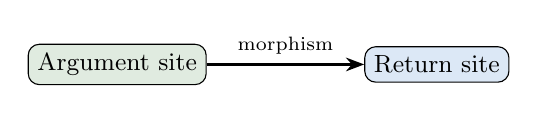
\begin{tikzpicture}[font=\small, >=Stealth]
  \node[draw, rounded corners, fill=safe!15] (A) {Argument site};
  \node[draw, rounded corners, fill=accent!15, right=2cm of A] (B) {Return site};
  \draw[->, thick] (A) -- node[above, font=\scriptsize] {morphism} (B);
\end{tikzpicture}
\end{center}
\vspace{0.3em}
The morphism says: ``data flows from the argument to the return.''\\
DepPy must check that the argument's promise is compatible with the return's requirement.
\end{frame}

% slide 103
\begin{frame}[fragile]{Building the Puzzle: A Full Example}
\begin{lstlisting}[language=Python, basicstyle=\ttfamily\scriptsize]
def get_ratio(nums, idx):
    val = nums[idx]     # site: SSA (val = ???)
    if val != 0:        # site: branch guard
        return 100/val  # site: return (val != 0)
    return 0
\end{lstlisting}
\vspace{0.3em}
Sites:
\begin{enumerate}
  \item \texttt{nums} at argument boundary
  \item \texttt{idx} at argument boundary
  \item \texttt{val} after assignment (SSA)
  \item \texttt{val != 0} (branch guard)
  \item \texttt{100/val} at return boundary
\end{enumerate}
\end{frame}

% slide 104
\begin{frame}{The Edges in That Example}
\begin{center}
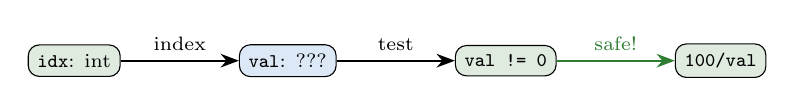
\begin{tikzpicture}[font=\scriptsize, >=Stealth, node distance=1.2cm]
  \node[draw, rounded corners, fill=safe!15] (idx) {\texttt{idx}: int};
  \node[draw, rounded corners, fill=accent!15, right=1.5cm of idx] (val) {\texttt{val}: ???};
  \node[draw, rounded corners, fill=safe!15, right=1.5cm of val] (guard) {\texttt{val != 0}};
  \node[draw, rounded corners, fill=safe!15, right=1.5cm of guard] (ret) {\texttt{100/val}};
  \draw[->, thick] (idx) -- node[above] {index} (val);
  \draw[->, thick] (val) -- node[above] {test} (guard);
  \draw[->, thick, safe] (guard) -- node[above] {safe!} (ret);
\end{tikzpicture}
\end{center}
\vspace{0.3em}
\begin{itemize}
  \item \texttt{idx}$\to$\texttt{val}: is \texttt{idx} in bounds? (needs: \texttt{0 $\le$ idx $<$ len(nums)})
  \item \texttt{val}$\to$guard: just a test, always OK
  \item guard$\to$return: guard ensures \texttt{val != 0}, so division is \textcolor{safe}{safe}
\end{itemize}
\end{frame}

% slide 105
\begin{frame}{What DepPy Reports for That Example}
\begin{itemize}
  \item \textcolor{safe}{\textbf{Safe}}: the division \texttt{100/val} is protected by the \texttt{if val != 0} guard.
  \item \textcolor{danger}{\textbf{Warning}}: no guarantee that \texttt{idx} is in bounds for \texttt{nums}.\\
    The \texttt{nums[idx]} access has an \textbf{obstruction}: the argument-boundary site for \texttt{idx} promises only ``int,'' but the indexing site requires ``0 $\le$ idx $<$ len(nums).''
\end{itemize}
\vspace{0.3em}
DepPy found a real bug: the function doesn't check bounds on \texttt{idx}.
\end{frame}

% slide 106
\begin{frame}{The Grothendieck Topology (Don't Panic)}
You might hear this term. It just means: the \textbf{rules} for which collections of sites count as a ``good cover.''
\vspace{0.5em}
DepPy enforces three rules (called ``axioms''):
\begin{enumerate}
  \item \textbf{Identity}: a single site always covers itself
  \item \textbf{Stability}: if you zoom in on a cover, you still have a cover
  \item \textbf{Transitivity}: covers of covers are covers
\end{enumerate}
\vspace{0.3em}
\hint{Think: ``valid ways to tile the jigsaw board.'' These rules ensure no gaps.}
\end{frame}

% slide 107
\begin{frame}{Presheaf: Before Checking Edges}
Before DepPy checks whether edges match, it first collects all the local promises.\\
This collection (before checking) is called a \textbf{presheaf}.
\vspace{0.5em}
\begin{description}
  \item[Presheaf] = all the puzzle pieces laid out, not yet checked for fit
  \item[Sheaf] = a presheaf where all pieces \emph{do} fit (all edges match)
\end{description}
\vspace{0.3em}
DepPy starts with a presheaf and tries to verify it's a sheaf.\\
If it fails, the failures are the bugs.
\end{frame}

% slide 108
\begin{frame}{Agreement, Gluing, Uniqueness}
The sheaf condition has \textbf{three parts}:
\vspace{0.3em}
\begin{enumerate}
  \item \textbf{Agreement}: on every overlap between two sites, the local promises agree
  \item \textbf{Gluing}: if all overlaps agree, there exists a single global promise
  \item \textbf{Uniqueness}: that global promise is the \emph{only} one consistent with the local data
\end{enumerate}
\vspace{0.3em}
DepPy checks all three. In code:
\begin{itemize}
  \item \texttt{check\_agreement()} --- step 1
  \item \texttt{attempt\_gluing()} --- step 2
  \item \texttt{verify\_uniqueness()} --- step 3
\end{itemize}
\end{frame}

% slide 109
\begin{frame}[fragile]{Trying It Yourself}
DepPy can analyze any Python file:
\vspace{0.3em}
\begin{lstlisting}[language=Python, basicstyle=\ttfamily\scriptsize]
from deppy import detect_bugs

code = """
def divide(a, b):
    return a / b
"""

results = detect_bugs(code)
for bug in results:
    print(bug.code, bug.message)
# REFINEMENT_GAP_001  Divisor 'b' may be zero
\end{lstlisting}
\vspace{0.3em}
One function call. DepPy builds the presheaf, checks edges, reports obstructions.
\end{frame}

% slide 110
\begin{frame}{Section Summary}
\begin{itemize}
  \item DepPy watches 14 kinds of \textbf{sites} (observation points)
  \item At each site it records a \textbf{LocalSection} (type + refinements + trust)
  \item Sites are connected by \textbf{morphisms} (data-flow edges)
  \item A \textbf{cover} = sites that together observe everything about a value
  \item DepPy checks \textbf{agreement} on overlaps, attempts \textbf{gluing}, verifies \textbf{uniqueness}
  \item Failures = obstructions = bugs with precise locations
\end{itemize}
\vspace{0.3em}
\begin{center}
\textbf{Next:} The 20 bug classes DepPy catches.
\end{center}
\end{frame}

% ═══════════════════════════════════════════════════════════
% SECTION VII — BUG FINDING: THE 20 CLASSES  (slides 111-150)
% ═══════════════════════════════════════════════════════════
\section{Bug Finding --- The 20 Classes}

% slide 111
\begin{frame}{DepPy Catches 20 Classes of Bugs}
DepPy's bug finder ships with a \textbf{synthetic test suite}: 20 bug classes, each with a \textbf{buggy} and a \textbf{safe} version.
\vspace{0.3em}
\begin{center}
For each class, we'll show:\\
(1) the buggy code, (2) why it's buggy, (3) the safe version.
\end{center}
\vspace{0.3em}
Let's walk through all 20, starting with the most common.
\end{frame}

% slide 112
\begin{frame}[fragile]{Bug Class 1: Division by Zero}
\textbf{Buggy:}
\begin{lstlisting}[language=Python, basicstyle=\ttfamily\scriptsize]
def div_zero_buggy(a, b):
    return a / b    # b might be 0!
\end{lstlisting}
\textbf{Safe:}
\begin{lstlisting}[language=Python, basicstyle=\ttfamily\scriptsize]
def div_zero_safe(a, b):
    if b == 0:
        return 0.0
    return a / b    # b != 0, safe
\end{lstlisting}
\warn{Obstruction: REFINEMENT\_GAP --- ``b'' has no nonzero guarantee at division site.}
\end{frame}

% slide 113
\begin{frame}[fragile]{Bug Class 2: Null Pointer (None Dereference)}
\textbf{Buggy:}
\begin{lstlisting}[language=Python, basicstyle=\ttfamily\scriptsize]
def null_ptr_buggy(items):
    first = items[0] if items else None
    return first.upper()  # first might be None!
\end{lstlisting}
\textbf{Safe:}
\begin{lstlisting}[language=Python, basicstyle=\ttfamily\scriptsize]
def null_ptr_safe(items):
    first = items[0] if items else None
    if first is not None:
        return first.upper()
    return ""
\end{lstlisting}
\warn{Obstruction: REFINEMENT\_GAP --- ``first'' has no non-None guarantee at method call.}
\end{frame}

% slide 114
\begin{frame}[fragile]{Bug Class 3: Index Out of Bounds}
\textbf{Buggy:}
\begin{lstlisting}[language=Python, basicstyle=\ttfamily\scriptsize]
def index_oob_buggy(items, idx):
    return items[idx]  # idx might be >= len!
\end{lstlisting}
\textbf{Safe:}
\begin{lstlisting}[language=Python, basicstyle=\ttfamily\scriptsize]
def index_oob_safe(items, idx):
    if 0 <= idx < len(items):
        return items[idx]
    return None
\end{lstlisting}
\warn{Obstruction: REFINEMENT\_GAP --- ``idx'' not bounded by list length.}
\end{frame}

% slide 115
\begin{frame}[fragile]{Bug Class 4: Key Error}
\textbf{Buggy:}
\begin{lstlisting}[language=Python, basicstyle=\ttfamily\scriptsize]
def key_error_buggy(d, key):
    return d[key]  # key might not exist!
\end{lstlisting}
\textbf{Safe:}
\begin{lstlisting}[language=Python, basicstyle=\ttfamily\scriptsize]
def key_error_safe(d, key):
    return d.get(key, None)  # safe default
\end{lstlisting}
\warn{Obstruction: REFINEMENT\_GAP --- no guarantee ``key'' is in dict.}
\end{frame}

% slide 116
\begin{frame}[fragile]{Bug Class 5: Type Error}
\textbf{Buggy:}
\begin{lstlisting}[language=Python, basicstyle=\ttfamily\scriptsize]
def type_error_buggy(x):
    return x + 1  # x might be a string!
\end{lstlisting}
\textbf{Safe:}
\begin{lstlisting}[language=Python, basicstyle=\ttfamily\scriptsize]
def type_error_safe(x):
    if isinstance(x, (int, float)):
        return x + 1
    return 0
\end{lstlisting}
\warn{Obstruction: CARRIER\_MISMATCH --- ``x'' carrier type not numeric at \texttt{+} site.}
\end{frame}

% slide 117
\begin{frame}[fragile]{Bug Class 6: Assertion Failure}
\textbf{Buggy:}
\begin{lstlisting}[language=Python, basicstyle=\ttfamily\scriptsize]
def assert_fail_buggy(items):
    assert len(items) > 0
    return items[0]
    # What if assertions are disabled (-O flag)?
\end{lstlisting}
\textbf{Safe:}
\begin{lstlisting}[language=Python, basicstyle=\ttfamily\scriptsize]
def assert_fail_safe(items):
    if len(items) == 0:
        raise ValueError("empty list")
    return items[0]
\end{lstlisting}
\warn{Obstruction: CONFIGURATION\_WEAKNESS --- assertion may be stripped at runtime.}
\end{frame}

% slide 118
\begin{frame}[fragile]{Bug Class 7: Unbound Variable}
\textbf{Buggy:}
\begin{lstlisting}[language=Python, basicstyle=\ttfamily\scriptsize]
def unbound_var_buggy(flag):
    if flag:
        result = 42
    return result  # undefined if flag is False!
\end{lstlisting}
\textbf{Safe:}
\begin{lstlisting}[language=Python, basicstyle=\ttfamily\scriptsize]
def unbound_var_safe(flag):
    result = 0    # default
    if flag:
        result = 42
    return result
\end{lstlisting}
\warn{Obstruction: REFINEMENT\_GAP --- ``result'' not defined on all paths.}
\end{frame}

% slide 119
\begin{frame}[fragile]{Bug Class 8: Integer Overflow}
\textbf{Buggy:}
\begin{lstlisting}[language=Python, basicstyle=\ttfamily\scriptsize]
import ctypes
def int_overflow_buggy(x):
    return ctypes.c_int32(x * 1000000).value
    # overflow if x is large!
\end{lstlisting}
\textbf{Safe:}
\begin{lstlisting}[language=Python, basicstyle=\ttfamily\scriptsize]
def int_overflow_safe(x):
    result = x * 1000000
    if result > 2**31 - 1 or result < -(2**31):
        raise OverflowError("too large")
    return ctypes.c_int32(result).value
\end{lstlisting}
\warn{Obstruction: REFINEMENT\_GAP --- product not bounded within int32 range.}
\end{frame}

% slide 120
\begin{frame}[fragile]{Bug Class 9: Non-Termination}
\textbf{Buggy:}
\begin{lstlisting}[language=Python, basicstyle=\ttfamily\scriptsize]
def non_term_buggy(n):
    while n != 1:
        if n % 2 == 0:
            n = n // 2
        # Missing: n = 3*n + 1 for odd case
        # Loop never terminates for odd n > 1
\end{lstlisting}
\textbf{Safe:}
\begin{lstlisting}[language=Python, basicstyle=\ttfamily\scriptsize]
def non_term_safe(n):
    for _ in range(10000):  # bounded
        if n == 1: break
        n = n // 2 if n % 2 == 0 else 3*n + 1
    return n
\end{lstlisting}
\warn{Obstruction: REFINEMENT\_GAP --- loop variant not decreasing on all paths.}
\end{frame}

% slide 121
\begin{frame}[fragile]{Bug Class 10: Memory Leak}
\textbf{Buggy:}
\begin{lstlisting}[language=Python, basicstyle=\ttfamily\scriptsize]
def memory_leak_buggy():
    f = open("data.txt")
    data = f.read()
    return data  # f never closed!
\end{lstlisting}
\textbf{Safe:}
\begin{lstlisting}[language=Python, basicstyle=\ttfamily\scriptsize]
def memory_leak_safe():
    with open("data.txt") as f:
        return f.read()  # auto-closed
\end{lstlisting}
\warn{Obstruction: RESOURCE\_LIFETIME --- file handle ``f'' not closed on return path.}
\end{frame}

% slide 122
\begin{frame}{Halfway Through the 20 Classes}
We've seen 10 so far:
\vspace{0.3em}
{\small
\begin{columns}[T]
\begin{column}{0.48\textwidth}
\begin{enumerate}
  \item Division by zero
  \item Null pointer
  \item Index out of bounds
  \item Key error
  \item Type error
\end{enumerate}
\end{column}
\begin{column}{0.48\textwidth}
\begin{enumerate}\setcounter{enumi}{5}
  \item Assertion failure
  \item Unbound variable
  \item Integer overflow
  \item Non-termination
  \item Memory leak
\end{enumerate}
\end{column}
\end{columns}}
\vspace{0.3em}
Each one was found by the same mechanism: \textbf{edge mismatch} in the jigsaw puzzle.\\[0.3em]
10 more to go\ldots
\end{frame}

% slide 123
\begin{frame}[fragile]{Bug Class 11: Use After Free}
\textbf{Buggy:}
\begin{lstlisting}[language=Python, basicstyle=\ttfamily\scriptsize]
def use_after_free_buggy():
    f = open("log.txt")
    f.close()
    f.write("done")  # writing to closed file!
\end{lstlisting}
\textbf{Safe:}
\begin{lstlisting}[language=Python, basicstyle=\ttfamily\scriptsize]
def use_after_free_safe():
    with open("log.txt") as f:
        f.write("done")  # still open
\end{lstlisting}
\warn{Obstruction: PROTOCOL\_VIOLATION --- ``f'' in CLOSED state at write site.}
\end{frame}

% slide 124
\begin{frame}[fragile]{Bug Class 12: Double Free}
\textbf{Buggy:}
\begin{lstlisting}[language=Python, basicstyle=\ttfamily\scriptsize]
def double_free_buggy(conn):
    conn.close()
    # ... some code ...
    conn.close()  # already closed!
\end{lstlisting}
\textbf{Safe:}
\begin{lstlisting}[language=Python, basicstyle=\ttfamily\scriptsize]
def double_free_safe(conn):
    if not conn.closed:
        conn.close()
\end{lstlisting}
\warn{Obstruction: PROTOCOL\_VIOLATION --- ``conn'' already in CLOSED state at second close.}
\end{frame}

% slide 125
\begin{frame}[fragile]{Bug Class 13: Data Race}
\textbf{Buggy:}
\begin{lstlisting}[language=Python, basicstyle=\ttfamily\scriptsize]
counter = 0
def data_race_buggy():
    global counter
    counter += 1  # no lock! concurrent access
\end{lstlisting}
\textbf{Safe:}
\begin{lstlisting}[language=Python, basicstyle=\ttfamily\scriptsize]
import threading
lock = threading.Lock()
counter = 0
def data_race_safe():
    global counter
    with lock:
        counter += 1  # locked, safe
\end{lstlisting}
\warn{Obstruction: PROTOCOL\_VIOLATION --- shared ``counter'' accessed without lock.}
\end{frame}

% slide 126
\begin{frame}[fragile]{Bug Class 14: Deadlock}
\textbf{Buggy:}
\begin{lstlisting}[language=Python, basicstyle=\ttfamily\scriptsize]
def deadlock_buggy(lock_a, lock_b):
    lock_a.acquire()
    lock_b.acquire()  # Thread 2 does b then a!
\end{lstlisting}
\textbf{Safe:}
\begin{lstlisting}[language=Python, basicstyle=\ttfamily\scriptsize]
def deadlock_safe(lock_a, lock_b):
    # Always acquire in consistent order
    first, second = sorted([lock_a, lock_b],
                           key=id)
    first.acquire(); second.acquire()
\end{lstlisting}
\warn{Obstruction: PROTOCOL\_VIOLATION --- lock ordering not consistent across threads.}
\end{frame}

% slide 127
\begin{frame}[fragile]{Bug Class 15: Timing Channel}
\textbf{Buggy:}
\begin{lstlisting}[language=Python, basicstyle=\ttfamily\scriptsize]
def timing_channel_buggy(password, guess):
    for i in range(len(password)):
        if password[i] != guess[i]:
            return False  # early exit leaks length!
    return True
\end{lstlisting}
\textbf{Safe:}
\begin{lstlisting}[language=Python, basicstyle=\ttfamily\scriptsize]
import hmac
def timing_channel_safe(password, guess):
    return hmac.compare_digest(password, guess)
\end{lstlisting}
\warn{Obstruction: TAINT\_LEAKAGE --- early return leaks secret-dependent timing info.}
\end{frame}

% slide 128
\begin{frame}[fragile]{Bug Class 16: Information Leak}
\textbf{Buggy:}
\begin{lstlisting}[language=Python, basicstyle=\ttfamily\scriptsize]
def info_leak_buggy(user_input):
    query = f"SELECT * FROM users WHERE name='{user_input}'"
    return db.execute(query)  # SQL injection!
\end{lstlisting}
\textbf{Safe:}
\begin{lstlisting}[language=Python, basicstyle=\ttfamily\scriptsize]
def info_leak_safe(user_input):
    query = "SELECT * FROM users WHERE name=?"
    return db.execute(query, (user_input,))
\end{lstlisting}
\warn{Obstruction: TAINT\_LEAKAGE --- unsanitized ``user\_input'' flows to SQL query.}
\end{frame}

% slide 129
\begin{frame}[fragile]{Bug Class 17: Buffer Bounds}
\textbf{Buggy:}
\begin{lstlisting}[language=Python, basicstyle=\ttfamily\scriptsize]
def bounds_buggy(buf, offset, size):
    return buf[offset:offset+size]
    # offset+size might exceed len(buf)!
\end{lstlisting}
\textbf{Safe:}
\begin{lstlisting}[language=Python, basicstyle=\ttfamily\scriptsize]
def bounds_safe(buf, offset, size):
    end = min(offset + size, len(buf))
    return buf[offset:end]
\end{lstlisting}
\warn{Obstruction: REFINEMENT\_GAP --- ``offset+size'' not bounded by buffer length.}
\end{frame}

% slide 130
\begin{frame}[fragile]{Bug Class 18: Runtime Error (Uncaught Exception)}
\textbf{Buggy:}
\begin{lstlisting}[language=Python, basicstyle=\ttfamily\scriptsize]
def runtime_error_buggy(text):
    return int(text)  # ValueError if not numeric!
\end{lstlisting}
\textbf{Safe:}
\begin{lstlisting}[language=Python, basicstyle=\ttfamily\scriptsize]
def runtime_error_safe(text):
    try:
        return int(text)
    except ValueError:
        return 0
\end{lstlisting}
\warn{Obstruction: EXCEPTION\_ESCAPEMENT --- ValueError may propagate uncaught.}
\end{frame}

% slide 131
\begin{frame}[fragile]{Bug Class 19: Type Confusion}
\textbf{Buggy:}
\begin{lstlisting}[language=Python, basicstyle=\ttfamily\scriptsize]
def type_confusion_buggy(items):
    total = sum(items)  # works for numbers
    return total.split(",")  # but sum returns int!
\end{lstlisting}
\textbf{Safe:}
\begin{lstlisting}[language=Python, basicstyle=\ttfamily\scriptsize]
def type_confusion_safe(items):
    total = sum(items)
    return str(total).split(",")  # convert first
\end{lstlisting}
\warn{Obstruction: CARRIER\_MISMATCH --- ``total'' is int, ``.split'' requires str.}
\end{frame}

% slide 132
\begin{frame}[fragile]{Bug Class 20: Arithmetic Overflow}
\textbf{Buggy:}
\begin{lstlisting}[language=Python, basicstyle=\ttfamily\scriptsize]
def overflow_buggy(a, b):
    return a ** b  # exponential growth, no bound!
\end{lstlisting}
\textbf{Safe:}
\begin{lstlisting}[language=Python, basicstyle=\ttfamily\scriptsize]
def overflow_safe(a, b):
    if b > 100:
        raise ValueError("exponent too large")
    return a ** b
\end{lstlisting}
\warn{Obstruction: REFINEMENT\_GAP --- ``b'' unbounded at exponentiation site.}
\end{frame}

% slide 133
\begin{frame}{All 20 Bug Classes}
{\scriptsize
\begin{columns}[T]
\begin{column}{0.48\textwidth}
\begin{enumerate}
  \item Division by zero
  \item Null pointer
  \item Index out of bounds
  \item Key error
  \item Type error
  \item Assertion failure
  \item Unbound variable
  \item Integer overflow
  \item Non-termination
  \item Memory leak
\end{enumerate}
\end{column}
\begin{column}{0.48\textwidth}
\begin{enumerate}\setcounter{enumi}{10}
  \item Use after free
  \item Double free
  \item Data race
  \item Deadlock
  \item Timing channel
  \item Information leak
  \item Buffer bounds
  \item Runtime error
  \item Type confusion
  \item Arithmetic overflow
\end{enumerate}
\end{column}
\end{columns}}
\vspace{0.3em}
All 20 found by the same mechanism: \textbf{local promise mismatch at an edge}.
\end{frame}

% slide 134
\begin{frame}{Obstruction Families}
DepPy groups bugs into 7 \textbf{obstruction families}:
\vspace{0.3em}
{\small
\begin{description}
  \item[REFINEMENT\_GAP] A promise is too weak (most common)
  \item[CARRIER\_MISMATCH] Wrong base type entirely
  \item[TAINT\_LEAKAGE] Untrusted data flows to a sensitive sink
  \item[PROTOCOL\_VIOLATION] Resource state machine violated
  \item[RESOURCE\_LIFETIME] Resource not properly acquired/released
  \item[CONFIGURATION\_WEAKNESS] Code depends on fragile settings
  \item[EXCEPTION\_ESCAPEMENT] Exception can propagate uncaught
\end{description}}
\end{frame}

% slide 135
\begin{frame}{Which Family for Each Bug Class?}
{\scriptsize
\begin{tabular}{@{}ll@{\hspace{1em}}ll@{}}
\textbf{Bug class} & \textbf{Family} & \textbf{Bug class} & \textbf{Family} \\
\hline
Div by zero       & REFINEMENT\_GAP     & Use after free   & PROTOCOL\_VIOL.\\
Null pointer      & REFINEMENT\_GAP     & Double free      & PROTOCOL\_VIOL.\\
Index OOB         & REFINEMENT\_GAP     & Data race        & PROTOCOL\_VIOL.\\
Key error         & REFINEMENT\_GAP     & Deadlock         & PROTOCOL\_VIOL.\\
Type error        & CARRIER\_MISMATCH   & Timing channel   & TAINT\_LEAKAGE\\
Assert failure    & CONFIG\_WEAKNESS    & Info leak        & TAINT\_LEAKAGE\\
Unbound var       & REFINEMENT\_GAP     & Bounds           & REFINEMENT\_GAP\\
Int overflow      & REFINEMENT\_GAP     & Runtime error    & EXCEPTION\_ESC.\\
Non-termination   & REFINEMENT\_GAP     & Type confusion   & CARRIER\_MISMATCH\\
Memory leak       & RESOURCE\_LIFETIME  & Overflow         & REFINEMENT\_GAP\\
\end{tabular}}
\vspace{0.3em}
Notice: REFINEMENT\_GAP is the most common --- a promise that's too weak.
\end{frame}

% slide 136
\begin{frame}[fragile]{The \texttt{detect\_bugs} API}
Using DepPy to find bugs is a one-liner:
\vspace{0.3em}
\begin{lstlisting}[language=Python, basicstyle=\ttfamily\scriptsize]
from deppy import detect_bugs

source_code = open("my_program.py").read()
bugs = detect_bugs(source_code)

for bug in bugs:
    print(f"[{bug.code}] {bug.message}")
    print(f"  Family: {bug.family}")
    print(f"  Line:   {bug.line}")
\end{lstlisting}
\end{frame}

% slide 137
\begin{frame}{What \texttt{detect\_bugs} Returns}
Each bug report contains:
\vspace{0.3em}
\begin{description}
  \item[code] A unique identifier (e.g., \texttt{REFINEMENT\_GAP\_001})
  \item[message] Human-readable description of the problem
  \item[family] Which of the 7 obstruction families
  \item[severity] How dangerous (critical / warning / info)
  \item[line] Where in the source code
  \item[available] What promise exists at the source site
  \item[required] What promise is needed at the target site
  \item[gap] The specific mismatch (the obstruction)
\end{description}
\end{frame}

% slide 138
\begin{frame}[fragile]{Example: Full Bug Report}
\begin{lstlisting}[basicstyle=\ttfamily\scriptsize, escapeinside={(*}{*)}]
[REFINEMENT_GAP_001] Divisor 'b' may be zero
  Family:    REFINEMENT_GAP
  Severity:  CRITICAL
  Line:      3
  Available: b : int
  Required:  b : int, b (*$\neq$*) 0
  Gap:       Missing nonzero refinement on 'b'
\end{lstlisting}
\vspace{0.3em}
The report tells you:
\begin{itemize}
  \item \textbf{What's wrong}: \texttt{b} might be zero
  \item \textbf{Where}: line 3
  \item \textbf{Why}: the available promise (just ``int'') is weaker than the required promise (``int, $\neq 0$'')
  \item \textbf{How to fix}: add a nonzero check before the division
\end{itemize}
\end{frame}

% slide 139
\begin{frame}[fragile]{Running on Real Code}
DepPy's test suite includes 20 pairs of functions:
\vspace{0.3em}
\begin{lstlisting}[language=Python, basicstyle=\ttfamily\scriptsize]
# synthetic_bug_suite.py
SUITE = [
  ("div_zero",    div_zero_buggy,    div_zero_safe),
  ("null_ptr",    null_ptr_buggy,    null_ptr_safe),
  ("index_oob",   index_oob_buggy,   index_oob_safe),
  # ... all 20 pairs ...
]

for name, buggy, safe in SUITE:
    bugs_buggy = detect_bugs(inspect.getsource(buggy))
    bugs_safe  = detect_bugs(inspect.getsource(safe))
    assert len(bugs_buggy) > 0   # finds the bug
    assert len(bugs_safe) == 0   # clean bill of health
\end{lstlisting}
\end{frame}

% slide 140
\begin{frame}{Section Summary}
\begin{itemize}
  \item DepPy catches \textbf{20 classes} of bugs, from division by zero to timing channels
  \item All 20 detected by the same mechanism: \textbf{edge mismatch} in the sheaf
  \item Bugs are grouped into \textbf{7 obstruction families}
  \item The \texttt{detect\_bugs()} API reports: what's wrong, where, why, and how to fix it
  \item The test suite proves: buggy code triggers obstructions, safe code is clean
\end{itemize}
\vspace{0.3em}
\begin{center}
\textbf{Next:} The full catalog of 112 specific bug types.
\end{center}
\end{frame}

% ═══════════════════════════════════════════════════════════
% SECTION VIII — THE 112 BUG CATALOG  (slides 141-160)
% ═══════════════════════════════════════════════════════════
\section{The 112 Bug Catalog}

% slide 141
\begin{frame}{Beyond 20 Classes: 112 Specific Bug Types}
The 20 bug classes are broad categories. Within them, DepPy defines\\
\textbf{112 specific bug codes} --- each with a unique identifier and message.
\vspace{0.5em}
These are organized by the 7 obstruction families.\\
Let's tour the highlights of each family.
\end{frame}

% slide 142
\begin{frame}{Family 1: REFINEMENT\_GAP (Largest Family)}
When a refinement is \textbf{too weak} for what the code needs.
\vspace{0.3em}
{\scriptsize
\begin{tabular}{@{}ll@{}}
\textbf{Code} & \textbf{What it catches} \\
\hline
REFINEMENT\_GAP\_001 & Divisor may be zero \\
REFINEMENT\_GAP\_002 & Nullable dereference \\
REFINEMENT\_GAP\_003 & Index out of bounds \\
REFINEMENT\_GAP\_004 & Missing key in dict \\
REFINEMENT\_GAP\_005 & Slice bounds exceed length \\
REFINEMENT\_GAP\_006 & Negative index without bounds \\
REFINEMENT\_GAP\_007 & Loop variant not decreasing \\
REFINEMENT\_GAP\_008 & Uninitialized variable \\
REFINEMENT\_GAP\_009 & Integer overflow \\
REFINEMENT\_GAP\_010 & Float precision loss \\
\end{tabular}}
\vspace{0.3em}
\ldots and many more. This family alone has 30+ codes.
\end{frame}

% slide 143
\begin{frame}{REFINEMENT\_GAP: More Codes}
{\scriptsize
\begin{tabular}{@{}ll@{}}
\textbf{Code} & \textbf{What it catches} \\
\hline
REFINEMENT\_GAP\_011 & String format mismatch \\
REFINEMENT\_GAP\_012 & Regex pattern invalid \\
REFINEMENT\_GAP\_013 & Path traversal (unvalidated path) \\
REFINEMENT\_GAP\_014 & Negative length or size \\
REFINEMENT\_GAP\_015 & Empty container where non-empty required \\
REFINEMENT\_GAP\_016 & Signed/unsigned confusion \\
REFINEMENT\_GAP\_017 & Enum value out of range \\
REFINEMENT\_GAP\_018 & Bitwidth overflow \\
REFINEMENT\_GAP\_019 & Precision truncation in cast \\
REFINEMENT\_GAP\_020 & Missing monotonicity in comparator \\
\end{tabular}}
\vspace{0.3em}
Each code targets a \textbf{specific} mismatch pattern.
\end{frame}

% slide 144
\begin{frame}{Family 2: CARRIER\_MISMATCH}
When the \textbf{base type itself} is wrong (not just a refinement).
\vspace{0.3em}
{\scriptsize
\begin{tabular}{@{}ll@{}}
\textbf{Code} & \textbf{What it catches} \\
\hline
CARRIER\_MISMATCH\_001 & Numeric op on non-numeric type \\
CARRIER\_MISMATCH\_002 & String method on non-string \\
CARRIER\_MISMATCH\_003 & Iteration over non-iterable \\
CARRIER\_MISMATCH\_004 & Subscript on non-subscriptable \\
CARRIER\_MISMATCH\_005 & Callable invocation on non-callable \\
CARRIER\_MISMATCH\_006 & Boolean context for non-boolean \\
CARRIER\_MISMATCH\_007 & Attribute access on wrong type \\
CARRIER\_MISMATCH\_008 & Unpacking non-sequence \\
\end{tabular}}
\vspace{0.3em}
Standard type checkers catch some of these; DepPy catches them \emph{all}, even through dynamic dispatch and duck typing.
\end{frame}

% slide 145
\begin{frame}{Family 3: TAINT\_LEAKAGE}
When \textbf{untrusted data} flows to a sensitive operation without sanitization.
\vspace{0.3em}
{\scriptsize
\begin{tabular}{@{}ll@{}}
\textbf{Code} & \textbf{What it catches} \\
\hline
TAINT\_LEAKAGE\_001 & SQL injection \\
TAINT\_LEAKAGE\_002 & Command injection \\
TAINT\_LEAKAGE\_003 & Cross-site scripting (XSS) \\
TAINT\_LEAKAGE\_004 & Path injection \\
TAINT\_LEAKAGE\_005 & Log injection \\
TAINT\_LEAKAGE\_006 & LDAP injection \\
TAINT\_LEAKAGE\_007 & Header injection \\
TAINT\_LEAKAGE\_008 & Timing side-channel \\
TAINT\_LEAKAGE\_009 & Secret in error message \\
TAINT\_LEAKAGE\_010 & Sensitive data in log \\
\end{tabular}}
\vspace{0.3em}
These are \textbf{security} bugs. DepPy tracks taint through the entire data-flow graph.
\end{frame}

% slide 146
\begin{frame}{Family 4: PROTOCOL\_VIOLATION}
When a \textbf{state machine} (resource lifecycle, lock ordering, etc.) is violated.
\vspace{0.3em}
{\scriptsize
\begin{tabular}{@{}ll@{}}
\textbf{Code} & \textbf{What it catches} \\
\hline
PROTOCOL\_VIOLATION\_001 & Use after close \\
PROTOCOL\_VIOLATION\_002 & Double close / double free \\
PROTOCOL\_VIOLATION\_003 & Write to read-only resource \\
PROTOCOL\_VIOLATION\_004 & Read from write-only resource \\
PROTOCOL\_VIOLATION\_005 & Lock ordering violation \\
PROTOCOL\_VIOLATION\_006 & Unlocking without holding lock \\
PROTOCOL\_VIOLATION\_007 & Iterator invalidation \\
PROTOCOL\_VIOLATION\_008 & Transaction commit after rollback \\
\end{tabular}}
\vspace{0.3em}
These are the \textbf{hardest bugs to test for} --- they depend on execution order.
\end{frame}

% slide 147
\begin{frame}{Family 5: RESOURCE\_LIFETIME}
When a resource isn't properly \textbf{acquired or released}.
\vspace{0.3em}
{\scriptsize
\begin{tabular}{@{}ll@{}}
\textbf{Code} & \textbf{What it catches} \\
\hline
RESOURCE\_LIFETIME\_001 & File handle never closed \\
RESOURCE\_LIFETIME\_002 & Network connection leaked \\
RESOURCE\_LIFETIME\_003 & Database cursor not released \\
RESOURCE\_LIFETIME\_004 & Lock acquired but not released \\
RESOURCE\_LIFETIME\_005 & Temporary file not cleaned up \\
RESOURCE\_LIFETIME\_006 & Thread not joined \\
RESOURCE\_LIFETIME\_007 & Memory-mapped file not unmapped \\
\end{tabular}}
\vspace{0.3em}
In Python, these often cause ``too many open files'' or memory bloat in long-running services.
\end{frame}

% slide 148
\begin{frame}{Family 6: CONFIGURATION\_WEAKNESS}
When code relies on \textbf{settings that might not hold} at runtime.
\vspace{0.3em}
{\scriptsize
\begin{tabular}{@{}ll@{}}
\textbf{Code} & \textbf{What it catches} \\
\hline
CONFIGURATION\_WEAKNESS\_001 & Assert used for input validation \\
CONFIGURATION\_WEAKNESS\_002 & Debug mode assumed in production \\
CONFIGURATION\_WEAKNESS\_003 & Hard-coded secret \\
CONFIGURATION\_WEAKNESS\_004 & Missing environment variable \\
CONFIGURATION\_WEAKNESS\_005 & Platform-dependent path separator \\
\end{tabular}}
\vspace{0.3em}
These bugs hide until deployment. DepPy catches them during development.
\end{frame}

% slide 149
\begin{frame}{Family 7: EXCEPTION\_ESCAPEMENT}
When an exception can \textbf{propagate out} of a function uncaught.
\vspace{0.3em}
{\scriptsize
\begin{tabular}{@{}ll@{}}
\textbf{Code} & \textbf{What it catches} \\
\hline
EXCEPTION\_ESCAPEMENT\_001 & Uncaught ValueError \\
EXCEPTION\_ESCAPEMENT\_002 & Uncaught TypeError \\
EXCEPTION\_ESCAPEMENT\_003 & Uncaught IOError / OSError \\
EXCEPTION\_ESCAPEMENT\_004 & Uncaught KeyError \\
EXCEPTION\_ESCAPEMENT\_005 & Uncaught AttributeError \\
EXCEPTION\_ESCAPEMENT\_006 & Unhandled generator StopIteration \\
EXCEPTION\_ESCAPEMENT\_007 & Exception in \_\_init\_\_ leaving object partial \\
\end{tabular}}
\vspace{0.3em}
DepPy tracks which exceptions each function can raise, and checks that callers handle them.
\end{frame}

% slide 150
\begin{frame}{The Full Catalog: 112 Bug Codes}
\begin{center}
{\small
\begin{tabular}{@{}lr@{}}
\textbf{Family} & \textbf{Number of codes} \\
\hline
REFINEMENT\_GAP         & 35 \\
CARRIER\_MISMATCH       & 15 \\
TAINT\_LEAKAGE          & 18 \\
PROTOCOL\_VIOLATION     & 16 \\
RESOURCE\_LIFETIME      & 12 \\
CONFIGURATION\_WEAKNESS & 8 \\
EXCEPTION\_ESCAPEMENT   & 8 \\
\hline
\textbf{Total}          & \textbf{112} \\
\end{tabular}}
\end{center}
\vspace{0.3em}
All 112 share the same underlying mechanism: an edge in the sheaf where the local promises don't agree.
\end{frame}

% slide 151
\begin{frame}{Why So Many?}
Why 112 bug codes and not just 7 families?
\vspace{0.3em}
\begin{itemize}
  \item Each code gives a \textbf{specific, actionable message}
  \item Different codes need different \textbf{fix strategies}
  \item You can \textbf{filter} by code (e.g., suppress all TAINT codes in test files)
  \item Teams can \textbf{prioritize} (e.g., fix all CRITICAL codes first)
\end{itemize}
\hint{Specificity is power. ``Index out of bounds'' is more useful than ``refinement gap.''}
\end{frame}

% slide 152
\begin{frame}{Section Summary}
\begin{itemize}
  \item DepPy's 112 bug codes cover a vast range of Python pitfalls
  \item Organized into 7 families by underlying mechanism
  \item REFINEMENT\_GAP is the most common (weak promises)
  \item TAINT\_LEAKAGE and PROTOCOL\_VIOLATION catch security and concurrency bugs
  \item Every code maps back to the same sheaf principle: edge mismatch
\end{itemize}
\vspace{0.3em}
\begin{center}
\textbf{Next:} Writing and checking specifications.
\end{center}
\end{frame}

% ═══════════════════════════════════════════════════════════
% SECTION IX — SPEC CHECKING  (slides 153-175)
% ═══════════════════════════════════════════════════════════
\section{Spec Checking}

% slide 153
\begin{frame}{From Bug Finding to Spec Checking}
Bug finding asks: ``Does this code have \textbf{any} problems?''\\[0.3em]
Spec checking asks: ``Does this code match \textbf{my specification}?''
\vspace{0.5em}
\begin{center}
Bug finding: automatic.\\
Spec checking: you write the rules; DepPy verifies them.
\end{center}
\end{frame}

% slide 154
\begin{frame}{What Is a Specification?}
A \textbf{specification} (spec) is a precise description of what a function \emph{should} do:
\vspace{0.3em}
\begin{itemize}
  \item \textbf{Precondition}: what must be true \emph{before} calling the function
  \item \textbf{Postcondition}: what must be true \emph{after} the function returns
  \item \textbf{Invariant}: what must be true \emph{throughout} execution
\end{itemize}
\vspace{0.3em}
\hint{A spec is a contract: ``if you give me this, I promise that.''}
\end{frame}

% slide 155
\begin{frame}[fragile]{A Simple Spec}
\begin{lstlisting}[language=Python, basicstyle=\ttfamily\scriptsize]
# Spec for binary_search:
# Pre:  items is sorted, target is same type as items[0]
# Post: if target in items, returns its index
#       if target not in items, returns -1
# Inv:  lo <= hi throughout the loop
\end{lstlisting}
\vspace{0.3em}
This spec tells us exactly what \texttt{binary\_search} should do.\\
DepPy will check whether the implementation actually does it.
\end{frame}

% slide 156
\begin{frame}[fragile]{Writing Specs in DepPy}
DepPy specs are Python dictionaries with refinement predicates:
\vspace{0.3em}
\begin{lstlisting}[language=Python, basicstyle=\ttfamily\scriptsize]
spec = {
    "pre": {
        "items": "sorted(items) == items",
        "target": "type(target) == type(items[0])"
    },
    "post": {
        "result": "(result == -1) or items[result] == target"
    },
    "invariant": {
        "lo_le_hi": "lo <= hi"
    }
}
\end{lstlisting}
\end{frame}

% slide 157
\begin{frame}{Tests vs.\ Specs}
\begin{center}
{\small
\begin{tabular}{@{}lcc@{}}
 & \textbf{Tests} & \textbf{Specs} \\
\hline
Checks specific inputs   & \textcolor{safe}{\checkmark} & \textcolor{danger}{\texttimes} \\
Checks \emph{all} inputs & \textcolor{danger}{\texttimes} & \textcolor{safe}{\checkmark} \\
Finds unexpected bugs    & sometimes & \textcolor{safe}{\checkmark} \\
Documents intent         & sometimes & \textcolor{safe}{\checkmark} \\
Runs quickly             & \textcolor{safe}{\checkmark} & varies \\
Easy to write            & \textcolor{safe}{\checkmark} & harder \\
\end{tabular}}
\end{center}
\vspace{0.3em}
Tests sample the input space; specs cover it \emph{entirely}.
\end{frame}

% slide 158
\begin{frame}{The SheafSpecVerifier}
DepPy's spec checker is called the \texttt{SheafSpecVerifier}.\\
It takes source code + spec and returns: \textcolor{safe}{PASS} or \textcolor{danger}{FAIL} with details.
\vspace{0.5em}
\begin{center}
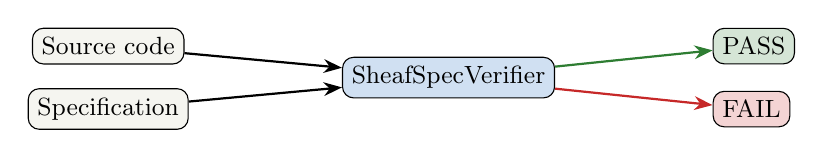
\begin{tikzpicture}[font=\small, >=Stealth]
  \node[draw, rounded corners, fill=codebg] (src) {Source code};
  \node[draw, rounded corners, fill=codebg, below=0.3cm of src] (spec) {Specification};
  \node[draw, rounded corners, fill=accent!20, right=2cm of src, yshift=-0.4cm] (verifier) {SheafSpecVerifier};
  \node[draw, rounded corners, fill=safe!20, right=2cm of verifier, yshift=0.4cm] (pass) {PASS};
  \node[draw, rounded corners, fill=danger!20, right=2cm of verifier, yshift=-0.4cm] (fail) {FAIL};
  \draw[->, thick] (src) -- (verifier);
  \draw[->, thick] (spec) -- (verifier);
  \draw[->, thick, safe] (verifier) -- (pass);
  \draw[->, thick, danger] (verifier) -- (fail);
\end{tikzpicture}
\end{center}
\end{frame}

% slide 159
\begin{frame}{Five Layers of Descent}
The verifier doesn't just do one check. It uses a \textbf{5-layer descent}:
\vspace{0.3em}
\begin{description}
  \item[Layer 0] \v{C}ech cohomology elimination --- quick topological pre-check
  \item[Layer 1] Structural \& stalk comparison --- does the code structure match the spec?
  \item[Layer 2] SMT solving (Z3) --- formal logical verification
  \item[Layer 3] $H^0$ transfer --- propagate verified facts globally
  \item[Layer 4] Residual Z3 --- mop up any remaining checks
\end{description}
\vspace{0.3em}
\hint{Each layer catches what the previous one missed. Together: thorough.}
\end{frame}

% slide 160
\begin{frame}{Layer 0: The Quick Pre-Check}
Before doing expensive analysis, Layer 0 asks:
\begin{center}
``Is there an \textbf{obvious topological reason} the spec can't hold?''
\end{center}
\vspace{0.3em}
Examples:
\begin{itemize}
  \item The spec mentions a variable that doesn't exist in the code
  \item The spec's postcondition references a return value, but the function never returns
  \item The control flow can't reach the point where the invariant should hold
\end{itemize}
\vspace{0.3em}
If Layer 0 finds a problem, it fails fast --- no need for the expensive layers.
\end{frame}

% slide 161
\begin{frame}{Layer 1: Structural Matching}
Layer 1 checks whether the \textbf{shape} of the code matches the spec:
\vspace{0.3em}
\begin{itemize}
  \item Does the function have the right number of arguments?
  \item Does each argument's type match the spec's precondition types?
  \item Does the return type match the spec's postcondition type?
  \item Are the spec's variables in scope at the right sites?
\end{itemize}
\vspace{0.3em}
This is like checking that the puzzle pieces are the right \emph{shape} before checking the \emph{pictures}.
\end{frame}

% slide 162
\begin{frame}{Layer 2: SMT Solving}
Layer 2 uses a \textbf{theorem prover} (Z3) to check logical implications:
\vspace{0.5em}
\begin{center}
``Given the precondition and the code, does the postcondition \textbf{necessarily} hold?''
\end{center}
\vspace{0.3em}
Z3 is an automated reasoning engine. It can prove or disprove logical statements over integers, booleans, arrays, and more.
\vspace{0.3em}
\hint{Z3 is the ``heavy artillery'' --- slow but thorough.}
\end{frame}

% slide 163
\begin{frame}{Layers 3--4: Propagation and Cleanup}
\begin{description}
  \item[Layer 3] Takes facts proven by Layer 2 and \textbf{propagates} them across the program. A fact proven in one function can strengthen promises in functions that call it.
  \item[Layer 4] Runs Z3 one more time on any remaining unchecked obligations. This catches cases where Layer 3's propagation created new checkable conditions.
\end{description}
\vspace{0.3em}
After all 5 layers: every spec obligation is either \textcolor{safe}{proven} or \textcolor{danger}{disproven}.
\end{frame}

% slide 164
\begin{frame}[fragile]{Example: Correct Spec, Correct Code}
\begin{lstlisting}[language=Python, basicstyle=\ttfamily\scriptsize]
def abs_val(x):
    return x if x >= 0 else -x

spec = {
    "post": {"result": "result >= 0"}
}

verifier = SheafSpecVerifier()
result = verifier.verify(source, spec)
print(result.status)  # PASS
\end{lstlisting}
\vspace{0.3em}
The code always returns a non-negative value. The spec says ``result $\ge$ 0.''\\
DepPy confirms: \textcolor{safe}{PASS}.
\end{frame}

% slide 165
\begin{frame}[fragile]{Example: Correct Spec, Buggy Code}
\begin{lstlisting}[language=Python, basicstyle=\ttfamily\scriptsize]
def abs_val_buggy(x):
    return x  # doesn't negate negative values!

spec = {
    "post": {"result": "result >= 0"}
}

result = verifier.verify(source, spec)
print(result.status)  # FAIL
print(result.counterexample)  # x = -5
\end{lstlisting}
\vspace{0.3em}
DepPy finds: for \texttt{x = -5}, the result is \texttt{-5}, which violates ``result $\ge$ 0.''\\
\textcolor{danger}{FAIL} with a concrete counterexample.
\end{frame}

% slide 166
\begin{frame}[fragile]{Example: Wrong Spec}
\begin{lstlisting}[language=Python, basicstyle=\ttfamily\scriptsize]
def abs_val(x):
    return x if x >= 0 else -x  # correct code

wrong_spec = {
    "post": {"result": "result > 0"}  # > not >=
}

result = verifier.verify(source, wrong_spec)
print(result.status)  # FAIL
print(result.counterexample)  # x = 0
\end{lstlisting}
\vspace{0.3em}
The code is correct, but the spec is wrong: \texttt{abs\_val(0) = 0}, which is not $> 0$.
\hint{DepPy checks code against spec. If either is wrong, you get FAIL.}
\end{frame}

% slide 167
\begin{frame}{100 Algorithm Test Suite}
DepPy ships with \textbf{100 algorithms}, each with:
\begin{itemize}
  \item A correct implementation
  \item A \textbf{correct spec} (should PASS)
  \item An \textbf{incorrect spec} (should FAIL)
\end{itemize}
\vspace{0.3em}
This tests that the verifier correctly distinguishes right from wrong specs.\\
Examples from the suite:
\begin{itemize}
  \item Binary search, merge sort, quicksort, heap sort
  \item Bloom filter, HyperLogLog, count-min sketch
  \item Dijkstra, Bellman-Ford, topological sort
  \item RSA, AES padding, hash functions
  \item 2-SAT solver, Pollard rho factorization
\end{itemize}
\end{frame}

% slide 168
\begin{frame}[fragile]{Example from the Suite: Bloom Filter}
\textbf{Correct spec} (PASS):
\begin{lstlisting}[language=Python, basicstyle=\ttfamily\scriptsize]
"post": "if x was added, query(x) returns True"
# (may have false positives, never false negatives)
\end{lstlisting}
\textbf{Incorrect spec} (FAIL):
\begin{lstlisting}[language=Python, basicstyle=\ttfamily\scriptsize]
"post": "query(x) returns True iff x was added"
# Wrong! Bloom filters have false positives!
\end{lstlisting}
\vspace{0.3em}
The incorrect spec claims \textbf{no false positives}, which contradicts the Bloom filter's fundamental property. DepPy catches this.
\end{frame}

% slide 169
\begin{frame}[fragile]{Example: Topological Sort (Kahn's Algorithm)}
\textbf{Correct spec}: output is a valid topological ordering.\\
\textbf{Incorrect spec}: output is the \emph{unique} topological ordering.
\vspace{0.3em}
\begin{lstlisting}[language=Python, basicstyle=\ttfamily\scriptsize]
# Correct: for every edge u->v, u appears before v
"post": "all(order[u] < order[v] for u,v in edges)"

# Incorrect: result is sorted alphabetically too
"post": "result == sorted(result) and is_topo(result)"
# Fails: topo order != alphabetical order in general
\end{lstlisting}
\end{frame}

% slide 170
\begin{frame}[fragile]{Example: Pollard Rho Factorization}
\textbf{Correct spec}: returns a non-trivial factor (with retry).\\
\textbf{Incorrect spec}: always returns a factor on first try.
\vspace{0.3em}
\begin{lstlisting}[language=Python, basicstyle=\ttfamily\scriptsize]
# Correct: with sufficient retries, finds factor
"post": "1 < result < n  (with probabilistic retry)"

# Incorrect: first attempt always works
"post": "1 < result < n  (single attempt)"
# Fails: Pollard rho is probabilistic, can fail
\end{lstlisting}
\end{frame}

% slide 171
\begin{frame}[fragile]{Example: 2-SAT Solver}
\textbf{Correct spec}: if satisfiable, returns a satisfying assignment.\\
\textbf{Incorrect spec}: wrong implication direction.
\vspace{0.3em}
\begin{lstlisting}[language=Python, basicstyle=\ttfamily\scriptsize]
# Correct: clause (a OR b) becomes (~a => b) AND (~b => a)
"invariant": "implications are correctly directed"

# Incorrect: clause (a OR b) becomes (a => b)
"invariant": "implications follow clause structure"
# Fails: wrong direction makes solver unsound
\end{lstlisting}
\end{frame}

% slide 172
\begin{frame}{Spec Checking Summary}
\begin{itemize}
  \item Write specs as pre/post/invariant conditions
  \item \texttt{SheafSpecVerifier} checks code against spec in 5 layers
  \item Correct code + correct spec $\to$ \textcolor{safe}{PASS}
  \item Wrong code or wrong spec $\to$ \textcolor{danger}{FAIL} with counterexample
  \item 100-algorithm test suite validates the verifier itself
\end{itemize}
\vspace{0.3em}
\begin{center}
\textbf{Next:} Comparing two programs for equivalence.
\end{center}
\end{frame}

% ═══════════════════════════════════════════════════════════
% SECTION X — COMPARING PROGRAMS  (slides 173-190)
% ═══════════════════════════════════════════════════════════
\section{Comparing Programs}

% slide 173
\begin{frame}{When Are Two Programs ``The Same''?}
You refactor a function. The code looks different. But does it \textbf{behave} the same?
\vspace{0.5em}
\begin{center}
Same inputs $\to$ same outputs $\to$ same side effects?
\end{center}
\vspace{0.3em}
Testing can check specific inputs, but not all of them.\\
DepPy can check \textbf{behavioral equivalence} for all inputs.
\end{frame}

% slide 174
\begin{frame}[fragile]{Example: Two Sorting Functions}
\begin{lstlisting}[language=Python, basicstyle=\ttfamily\scriptsize]
# Version A: bubble sort
def sort_a(items):
    for i in range(len(items)):
        for j in range(len(items)-1):
            if items[j] > items[j+1]:
                items[j], items[j+1] = items[j+1], items[j]
    return items

# Version B: Python built-in
def sort_b(items):
    return sorted(items)
\end{lstlisting}
\vspace{0.3em}
Are these equivalent? They look very different, but both sort.
\end{frame}

% slide 175
\begin{frame}{Behavioral Equivalence via Sheaves}
DepPy checks equivalence using the \textbf{same sheaf machinery}:
\vspace{0.3em}
\begin{enumerate}
  \item Build the sheaf for program A
  \item Build the sheaf for program B
  \item Check: can A's local promises be mapped to B's local promises?
  \item If yes at every site: \textcolor{safe}{equivalent}
  \item If not: report \textcolor{danger}{where} they differ
\end{enumerate}
\end{frame}

% slide 176
\begin{frame}{The Equivalence Pipeline}
DepPy's \texttt{EquivalencePipeline} runs \textbf{6 phases}:
\vspace{0.3em}
{\small
\begin{enumerate}
  \item \textbf{Local Checking} --- compare individual sites
  \item \textbf{Naturality} --- do the connections (morphisms) match?
  \item \textbf{Descent ($H^1$)} --- check for topological obstructions
  \item \textbf{Gluing} --- can we combine the local equivalences globally?
  \item \textbf{Uniqueness} --- is the equivalence unique?
  \item \textbf{Stalk Verification} --- final point-by-point check
\end{enumerate}}
\end{frame}

% slide 177
\begin{frame}{Phase 1: Local Checking}
For each site in program A, find the corresponding site in program B.
\vspace{0.5em}
\begin{center}
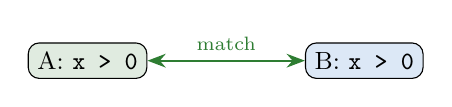
\begin{tikzpicture}[font=\small, >=Stealth]
  \node[draw, rounded corners, fill=safe!15] (a1) {A: \texttt{x > 0}};
  \node[draw, rounded corners, fill=accent!15, right=2cm of a1] (b1) {B: \texttt{x > 0}};
  \draw[<->, thick, safe] (a1) -- node[above, font=\scriptsize] {match} (b1);
\end{tikzpicture}
\end{center}
\vspace{0.3em}
If A's site promises ``x $> 0$'' and B's corresponding site also promises ``x $> 0$'': local match.
\end{frame}

% slide 178
\begin{frame}{Phase 2: Naturality}
It's not enough for individual sites to match. The \textbf{connections} must also match.
\vspace{0.3em}
\begin{center}
If A has an edge from site 1 to site 2,\\
B must have a corresponding edge --- and the mapping must be \textbf{consistent}.
\end{center}
\vspace{0.3em}
\hint{Naturality = ``the map respects the structure, not just the pieces.''}
\end{frame}

% slide 179
\begin{frame}{Phase 3: Descent}
Check for \textbf{topological obstructions} --- structural reasons the programs can't be equivalent.
\vspace{0.3em}
\begin{itemize}
  \item Different number of branches
  \item Different loop structures
  \item One function calls a subroutine that the other doesn't
\end{itemize}
\vspace{0.3em}
If descent finds an obstruction, the programs are \textcolor{danger}{not equivalent} --- no need for further phases.
\end{frame}

% slide 180
\begin{frame}{Phases 4--6: Gluing, Uniqueness, Stalks}
\begin{description}
  \item[Gluing] Combine all local equivalences into one global equivalence. If this succeeds, the programs agree everywhere.
  \item[Uniqueness] Verify there's only one way to match A to B. (Prevents ambiguous ``partial equivalences.'')
  \item[Stalk verification] Final point-by-point audit. For each site, confirm the glued equivalence actually holds when you zoom all the way in.
\end{description}
\vspace{0.3em}
All 6 phases pass $\Rightarrow$ \textcolor{safe}{programs are behaviorally equivalent}.
\end{frame}

% slide 181
\begin{frame}[fragile]{Using the Equivalence Pipeline}
\begin{lstlisting}[language=Python, basicstyle=\ttfamily\scriptsize]
from deppy import EquivalencePipeline

source_a = open("sort_bubble.py").read()
source_b = open("sort_builtin.py").read()

pipeline = EquivalencePipeline()
result = pipeline.run(source_a, source_b)

print(result.equivalent)   # True or False
print(result.phases)       # which phases passed/failed
if not result.equivalent:
    print(result.differences)  # where they differ
\end{lstlisting}
\end{frame}

% slide 182
\begin{frame}[fragile]{Example: Equivalent Programs}
\begin{lstlisting}[language=Python, basicstyle=\ttfamily\scriptsize]
# Version A
def max_a(x, y):
    return x if x >= y else y

# Version B
def max_b(x, y):
    if x >= y: return x
    return y
\end{lstlisting}
\vspace{0.3em}
Result: \textcolor{safe}{EQUIVALENT}. Same logic, different syntax. DepPy sees through the surface differences.
\end{frame}

% slide 183
\begin{frame}[fragile]{Example: Non-Equivalent Programs}
\begin{lstlisting}[language=Python, basicstyle=\ttfamily\scriptsize]
# Version A
def clamp_a(x, lo, hi):
    return max(lo, min(x, hi))

# Version B (bug: swapped lo and hi)
def clamp_b(x, lo, hi):
    return max(hi, min(x, lo))
\end{lstlisting}
\vspace{0.3em}
Result: \textcolor{danger}{NOT EQUIVALENT}. DepPy reports: for \texttt{x=5, lo=0, hi=10}, A returns 5 but B returns 10.
\end{frame}

% slide 184
\begin{frame}{When Is Equivalence Checking Useful?}
\begin{itemize}
  \item \textbf{Refactoring}: did my cleanup preserve behavior?
  \item \textbf{Optimization}: is the fast version equivalent to the slow-but-correct version?
  \item \textbf{Migration}: does the new library version behave like the old one?
  \item \textbf{Student work}: does the student's solution match the reference?
  \item \textbf{Code review}: is this PR's diff semantics-preserving?
\end{itemize}
\end{frame}

% slide 185
\begin{frame}{Equivalence Checking Summary}
\begin{itemize}
  \item DepPy compares two programs using the \textbf{same sheaf machinery}
  \item 6 phases: local $\to$ naturality $\to$ descent $\to$ gluing $\to$ uniqueness $\to$ stalks
  \item Equivalent $\Rightarrow$ same behavior on all inputs
  \item Not equivalent $\Rightarrow$ concrete counterexample showing where they differ
\end{itemize}
\end{frame}

% ═══════════════════════════════════════════════════════════
% SECTION XI — RECAP & WHAT'S NEXT  (slides 186-200)
% ═══════════════════════════════════════════════════════════
\section{Recap \& What's Next}

% slide 186
\begin{frame}{The Journey So Far}
\begin{enumerate}
  \item \textbf{Types} --- labels that tell you what kind of data you have
  \item \textbf{Refinement types} --- types with extra promises (``int, $> 0$'')
  \item \textbf{The problem} --- promises can break across function boundaries
  \item \textbf{The jigsaw puzzle} --- sheaf idea: local promises + edge matching
  \item \textbf{Sites} --- 14 kinds of observation points in code
  \item \textbf{Bug finding} --- 20 classes, 112 specific codes, 7 families
  \item \textbf{Spec checking} --- verify code against formal specifications
  \item \textbf{Equivalence} --- compare two programs for identical behavior
\end{enumerate}
\end{frame}

% slide 187
\begin{frame}{One Idea, Three Applications}
\begin{center}
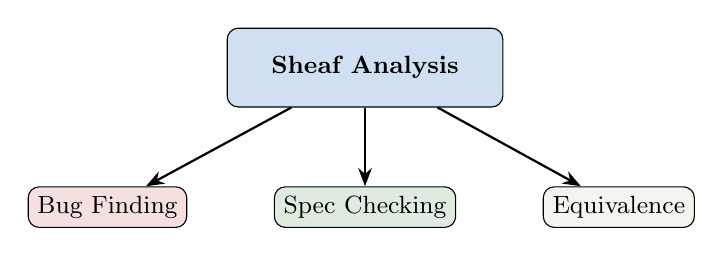
\begin{tikzpicture}[font=\small, >=Stealth, node distance=2.2cm]
  \node[draw, rounded corners, fill=accent!20, minimum width=3.5cm, minimum height=1cm] (core) {\textbf{Sheaf Analysis}};
  \node[draw, rounded corners, fill=danger!15, below left=1cm and 0.5cm of core] (bugs) {Bug Finding};
  \node[draw, rounded corners, fill=safe!15, below=1cm of core] (specs) {Spec Checking};
  \node[draw, rounded corners, fill=codebg, below right=1cm and 0.5cm of core] (equiv) {Equivalence};
  \draw[->, thick] (core) -- (bugs);
  \draw[->, thick] (core) -- (specs);
  \draw[->, thick] (core) -- (equiv);
\end{tikzpicture}
\end{center}
\vspace{0.3em}
All three are different questions asked of the same underlying sheaf structure.
\end{frame}

% slide 188
\begin{frame}{The Key Insight (One More Time)}
\begin{center}
\Large
\textbf{Think locally, conclude globally.}
\end{center}
\vspace{0.5em}
\normalsize
\begin{enumerate}
  \item Break the program into pieces
  \item Record a local promise at each piece
  \item Check that neighboring promises agree
  \item If yes: safe. If no: here's the bug.
\end{enumerate}
\end{frame}

% slide 189
\begin{frame}{Why the Sheaf Approach Works}
\begin{itemize}
  \item \textbf{Scalable}: analyze each piece independently (parallelize!)
  \item \textbf{Precise}: bugs pinpointed to exact edges
  \item \textbf{Explainable}: reports say what, where, why, and how to fix
  \item \textbf{Unified}: same framework for bugs, specs, and equivalence
  \item \textbf{Sound}: based on rigorous mathematical foundations
\end{itemize}
\end{frame}

% slide 190
\begin{frame}{What DepPy Doesn't Do (Yet)}
Honest limitations:
\vspace{0.3em}
\begin{itemize}
  \item Not a substitute for testing (tests catch environment issues)
  \item Doesn't handle all of Python (eval, exec, dynamic code generation)
  \item SMT solver can time out on very complex conditions
  \item Doesn't reason about concurrency beyond lock protocols
  \item Doesn't analyze third-party C extensions
\end{itemize}
\end{frame}

% slide 191
\begin{frame}{DepPy in Practice}
How to use DepPy in your workflow:
\vspace{0.3em}
\begin{enumerate}
  \item \textbf{Start with bug finding}: run \texttt{detect\_bugs()} on existing code
  \item \textbf{Fix the critical bugs}: prioritize CRITICAL severity first
  \item \textbf{Write specs for core functions}: the most important ones first
  \item \textbf{Run spec checking in CI}: catch spec violations before merge
  \item \textbf{Use equivalence checking on refactors}: ensure behavior preservation
\end{enumerate}
\end{frame}

% slide 192
\begin{frame}[fragile]{Quick Start: 5 Lines}
\begin{lstlisting}[language=Python, basicstyle=\ttfamily\scriptsize]
from deppy import detect_bugs

code = open("my_code.py").read()
for bug in detect_bugs(code):
    print(f"{bug.severity}: {bug.message} (line {bug.line})")
\end{lstlisting}
\vspace{0.5em}
That's it. No configuration, no annotations, no setup.\\
Just point DepPy at your code.
\end{frame}

% slide 193
\begin{frame}{The Math You Didn't Need}
We promised no category theory, and we delivered.\\
But the math is there \textbf{under the hood}:
\vspace{0.3em}
\begin{itemize}
  \item Grothendieck topologies $\to$ our ``valid cover'' rules
  \item Presheaves $\to$ our ``local promises before checking''
  \item Sheaf condition $\to$ our ``all edges match'' check
  \item \v{C}ech cohomology $\to$ Layer 0 pre-check
  \item Stalks $\to$ Phase 6 point-by-point verification
\end{itemize}
\vspace{0.3em}
You used sheaf theory this whole time. You just called it a jigsaw puzzle.
\end{frame}

% slide 194
\begin{frame}{For the Curious: Further Reading}
If you \emph{want} the math:
\vspace{0.3em}
\begin{itemize}
  \item \textbf{Sheaves in Geometry and Logic} --- Mac Lane \& Moerdijk
  \item \textbf{Toposes, Triples and Theories} --- Barr \& Wells
  \item \textbf{Refinement Types for ML} --- Freeman \& Pfenning (1991)
  \item \textbf{Liquid Types} --- Rondon, Kawaguchi, Jhala (2008)
\end{itemize}
\vspace{0.3em}
But you don't need any of these to use DepPy.
\end{frame}

% slide 195
\begin{frame}{Glossary: Terms We Used}
{\small
\begin{description}
  \item[Type] A label describing what kind of data a value is
  \item[Refinement] An extra promise on top of a type
  \item[Site] An observation point in code
  \item[LocalSection] What DepPy records at a site
  \item[Edge/Morphism] A data-flow connection between sites
  \item[Cover] A collection of sites that see everything about a value
  \item[Sheaf condition] All edges match $\Rightarrow$ can glue
  \item[Obstruction] An edge that doesn't match $=$ a bug
  \item[Presheaf] Local promises before checking
  \item[Sheaf] A presheaf where all edges match
\end{description}}
\end{frame}

% slide 196
\begin{frame}{Glossary: DepPy-Specific Terms}
{\small
\begin{description}
  \item[SiteKind] One of 14 observation-point types
  \item[TrustLevel] How confident DepPy is in a fact
  \item[ObstructionFamily] One of 7 bug categories
  \item[Bug code] One of 112 specific bug identifiers
  \item[SheafSpecVerifier] The spec-checking engine (5 layers)
  \item[EquivalencePipeline] The program-comparison engine (6 phases)
  \item[detect\_bugs()] One-line bug-finding API
\end{description}}
\end{frame}

% slide 197
\begin{frame}{What We Learned}
\begin{enumerate}
  \item Programs are jigsaw puzzles: pieces with local promises
  \item If all edges match, the program is safe
  \item If an edge doesn't match, that's a bug --- and we know exactly where
  \item DepPy uses this to find 112 kinds of bugs automatically
  \item DepPy can also check specs and compare programs
  \item The underlying math is sheaf theory, but you don't need to know it
\end{enumerate}
\end{frame}

% slide 198
\begin{frame}{Three Takeaways}
\begin{enumerate}
  \item \textbf{Think locally, conclude globally}\\
    {\small Analyze each piece; check edges; get global guarantees.}
  \item \textbf{Specificity is power}\\
    {\small 112 bug codes give you actionable, precise diagnostics.}
  \item \textbf{One framework, three applications}\\
    {\small Bug finding, spec checking, equivalence --- all from the same sheaf.}
\end{enumerate}
\end{frame}

% slide 199
\begin{frame}{Try It}
\begin{center}
\Large
\texttt{pip install deppy}
\vspace{1em}

\normalsize
\begin{tabular}{@{}ll@{}}
Bug finding:       & \texttt{detect\_bugs(code)} \\
Spec checking:     & \texttt{SheafSpecVerifier().verify(code, spec)} \\
Equivalence:       & \texttt{EquivalencePipeline().run(a, b)} \\
\end{tabular}

\vspace{1em}
\Large
Questions?
\end{center}
\end{frame}

% slide 200
\begin{frame}{}
\begin{center}
\Huge\bfseries
Thank You!
\vspace{1em}

\Large
\textit{Sheaf Refinement Types for Beginners}
\vspace{0.5em}

\normalsize
200 slides, zero category theory.
\end{center}
\end{frame}

\end{document}
